\documentclass[output=paper,colorlinks,citecolor=brown]{langscibook}
\ChapterDOI{10.5281/zenodo.17158180}
\author{Riccardo Orrico\orcid{0000-0001-9260-7210}\affiliation{Radboud University, Nijmegen} and Cristel Portes\orcid{0000-0002-1764-2945}\affiliation{Aix Marseille Université, Laboratoire Parole et Langage} and Mariapaola D'Imperio\orcid{0000-0001-5122-4555}\affiliation{Aix Marseille Université, Laboratoire Parole et Langage, CNRS}}
\title{The contribution of intonation in the conveyance of question bias} 
\abstract{The aim of this chapter is to address the issue of how meanings related to bias in polar questions are conveyed by intonation. We present an overview of previous studies conducted on two Romance languages, Italian and French. The review of these studies is used to show how intonation can be used in different languages to signal the presence and the polarity of question bias, as well as the source of information from which the bias stems. We also point out that future research on this topic should deal with, among other things, how gradient phonetic information maps onto meanings and the role of individual variability.}

\IfFileExists{../localcommands.tex}{
   \addbibresource{../localbibliography.bib}
   \usepackage{tabularx,multicol}
%	\setlength{\multicolsep}{6.0pt plus 2.0pt minus 2.0pt}
\usepackage{array} % for the 'm' column type
\usepackage{multirow}

%font:
\usepackage{siunitx}
\sisetup{group-digits=none}

\usepackage{textcomp} %emdash

%\usepackage{libertinus−otf}
%\setmainfont{Libertinus}

 
\usepackage{langsci-optional}
\usepackage{langsci-lgr}
\usepackage{langsci-gb4e}
\usepackage{langsci-basic}
\usepackage{langsci-affiliations}
\usepackage{langsci-branding}

\usepackage{url}
\urlstyle{same}
\usepackage{orcidlink}

%\usepackage{langsci-textipa}

\usepackage{amsmath}
\usepackage{amssymb}
\usepackage{stmaryrd}

%\usepackage{biblatex}%citation input! DO NOT CHANGE!
%\usepackage[american]{babel}
%\usepackage{csquotes}
%\usepackage[style=apa]{biblatex}
%\bibliographystyle{linquiry2}
%\usepackage[hidelinks, bookmarks=false, pdfstartview=FitH]{hyperref} %bookmarks=false, urlcolor=blue,

\usepackage{pifont} %checkmarks
%\usepackage{ulem}

%no new packages for 02.tex :

%\usepackage{setspace}
%\doublespacing
%\singlespacing


\usepackage{tikz-qtree}
\usepackage{tikz-qtree-compat}
\tikzset{every tree node/.style={align=center,anchor=north}}
%\usepackage{qtree,tree-dvips}%for trees, dvips won't work with figures unless figures are converted to .eps. make sure Typeset is set to "tex and DVI", not "pdftex" 
%\qtreecentertrue
\usepackage[linguistics]{forest}
\forestset{
fairly nice empty nodes/.style={
delay={where content={}
{shape=coordinate, for siblings={anchor=north}}{}},
for tree={s sep=4mm} }
            }


\usepackage[nameinlink]{cleveref} %for \Cref{}
% \usepackage{comment}
% \usepackage{color}
% \usepackage{subcaption}
\usepackage{subfigure}
% \usepackage{caption}
\usepackage{arydshln}

% \usepackage[scale=0.8]{FiraMono}

%\usepackage[export]{adjustbox}

%03.tex packages:
%\usepackage{linguex}%for examples

%04.tex packages:
\usepackage{cancel}
\usepackage{metre}
% \pagenumbering{roman}

%08.tex packages:
% \usepackage{xeCJK} %Chinese fonts
% \newfontfamily{\NotoSerifTC}{Noto Serif TC}
% \setCJKmainfont{Noto Serif TC}

   %for all .tex files (Affiliation setups):
\SetupAffiliations{ output in groups = false,
separator between two = {\bigskip\\},
separator between multiple = {\bigskip\\},
separator between final two = {\bigskip\\},
orcid placement=after
}

% ORCIDs in langsci-affiliations 
\definecolor{orcidlogocol}{cmyk}{0,0,0,1}
\RenewDocumentCommand{\LinkToORCIDinAffiliations}{ +m }
  {%
    \,\orcidlink{#1}%
  }

\makeatletter
\let\thetitle\@title
\let\theauthor\@author
\makeatother

\newcommand{\togglepaper}[1][0]{
   \bibliography{../localbibliography}
   \papernote{\scriptsize\normalfont
     \theauthor.
     \titleTemp.
     To appear in:
     E. Di Tor \& Herr Rausgeberin (ed.).
     Booktitle in localcommands.tex.
     Berlin: Language Science Press. [preliminary page numbering]
   }
   \pagenumbering{roman}
   \setcounter{chapter}{#1}
   \addtocounter{chapter}{-1}
}

\newbool{bookcompile}
\booltrue{bookcompile}
\newcommand{\bookorchapter}[2]{\ifbool{bookcompile}{#1}{#2}}

\newcommand{\cmark}{\ding{51}}%
\newcommand{\xmark}{\ding{55}}%

%for 01.tex:
\newcommand{\eval}[2]{\llbracket #1\rrbracket^{#2}}

%02.tex:
\newcommand{\smiley}{:)}

%03.tex:
\newcommand{\exa}{\ea}
%\renewcommand{\firstrefdash}{}%changes citations from, e.g., (2-a) to (2a)
\newcommand{\den}[2]{\ensuremath{\llbracket#1\rrbracket}\textsuperscript{\ensuremath{#2}}}
\newcommand{\citepos}[1]{\citeauthor{#1}'s (\citeyear{#1})}
\newcommand{\tp}[1]{\ensuremath{{\langle #1 \rangle}}}

\newcommand{\rise}{$\nearrow$\xspace}
\newcommand{\fall}{$\searrow$\xspace}
\newcommand{\notp}{\emph{not}-$p$\xspace}

%09.tex:
%\newcommand\den[1]{\ensuremath{[\![ #1 ]\!]}}
%\newcommand{\int}[1]{\ensuremath{\llbracket #1 \rrbracket}}

%13.tex:
\newcommand{\PreserveBackslash}[1]{\let\temp=\\#1\let\\=\temp}
% \newcolumntype{C}[1]{>{\PreserveBackslash\centering}p{#1}}
\newcolumntype{R}[1]{>{\PreserveBackslash\raggedleft}p{#1}}
\newcolumntype{L}[1]{>{\PreserveBackslash\raggedright}p{#1}}

\newcommand{\SB}{\textsubscript}
\newcommand{\SuB}{\textsuperscript}

\newcommand{\quotecite}[1]{\citeauthor{#1}'s (\citeyear*{#1})}

   %% hyphenation points for line breaks
%% Normally, automatic hyphenation in LaTeX is very good
%% If a word is mis-hyphenated, add it to this file
%%
%% add information to TeX file before \begin{document} with:
%% %% hyphenation points for line breaks
%% Normally, automatic hyphenation in LaTeX is very good
%% If a word is mis-hyphenated, add it to this file
%%
%% add information to TeX file before \begin{document} with:
%% %% hyphenation points for line breaks
%% Normally, automatic hyphenation in LaTeX is very good
%% If a word is mis-hyphenated, add it to this file
%%
%% add information to TeX file before \begin{document} with:
%% \include{localhyphenation}
\hyphenation{
    par-a-digm
}
\hyphenation{
que-stions
}
\hyphenation{
na-me-l-y
}
\hyphenation{
ge-ne-ra-tion
}
\hyphenation{
Hir-sch-berg}
\hyphenation{
stee-p-er
}
\hyphenation{
inter-ro-ga-tives
}
\hyphenation{
cons-truc-tion
}
\hyphenation{
p-u-sh-ed
}
\hyphenation{
A-mong
}
\hyphenation{
award-ed
}
\hyphenation{
synta-ctic
}
%\hyphenation{
%wh-ich
%}
\hyphenation{
call-ed
}
\hyphenation{
mo-no-po-lar
}
\hyphenation{
proso-dic
}
\hyphenation{
non-ve-ri-di-cal
}
\hyphenation{
Ro-me-ro
}
\hyphenation{
though
}
\hyphenation{
ra-ther
}
\hyphenation{
mo-da-li-ty
}
\hyphenation{
prag-ma-ti-cal-ly
}
\hyphenation{
trans-ver-sal
}
\hyphenation{
re-se-arch
}
\hyphenation{
clau-s-es
}
\hyphenation{
c-lau-se
}
\hyphenation{
spea-k-er
}
\hyphenation{
a-mon-g-st
}
\hyphenation{
th-rou-gh
}
\hyphenation{
ad-dres-see
}
\hyphenation{
mo-da-li-s-ed
}
\hyphenation{
Ja-mie-son}








\hyphenation{
    par-a-digm
}
\hyphenation{
que-stions
}
\hyphenation{
na-me-l-y
}
\hyphenation{
ge-ne-ra-tion
}
\hyphenation{
Hir-sch-berg}
\hyphenation{
stee-p-er
}
\hyphenation{
inter-ro-ga-tives
}
\hyphenation{
cons-truc-tion
}
\hyphenation{
p-u-sh-ed
}
\hyphenation{
A-mong
}
\hyphenation{
award-ed
}
\hyphenation{
synta-ctic
}
%\hyphenation{
%wh-ich
%}
\hyphenation{
call-ed
}
\hyphenation{
mo-no-po-lar
}
\hyphenation{
proso-dic
}
\hyphenation{
non-ve-ri-di-cal
}
\hyphenation{
Ro-me-ro
}
\hyphenation{
though
}
\hyphenation{
ra-ther
}
\hyphenation{
mo-da-li-ty
}
\hyphenation{
prag-ma-ti-cal-ly
}
\hyphenation{
trans-ver-sal
}
\hyphenation{
re-se-arch
}
\hyphenation{
clau-s-es
}
\hyphenation{
c-lau-se
}
\hyphenation{
spea-k-er
}
\hyphenation{
a-mon-g-st
}
\hyphenation{
th-rou-gh
}
\hyphenation{
ad-dres-see
}
\hyphenation{
mo-da-li-s-ed
}
\hyphenation{
Ja-mie-son}








\hyphenation{
    par-a-digm
}
\hyphenation{
que-stions
}
\hyphenation{
na-me-l-y
}
\hyphenation{
ge-ne-ra-tion
}
\hyphenation{
Hir-sch-berg}
\hyphenation{
stee-p-er
}
\hyphenation{
inter-ro-ga-tives
}
\hyphenation{
cons-truc-tion
}
\hyphenation{
p-u-sh-ed
}
\hyphenation{
A-mong
}
\hyphenation{
award-ed
}
\hyphenation{
synta-ctic
}
%\hyphenation{
%wh-ich
%}
\hyphenation{
call-ed
}
\hyphenation{
mo-no-po-lar
}
\hyphenation{
proso-dic
}
\hyphenation{
non-ve-ri-di-cal
}
\hyphenation{
Ro-me-ro
}
\hyphenation{
though
}
\hyphenation{
ra-ther
}
\hyphenation{
mo-da-li-ty
}
\hyphenation{
prag-ma-ti-cal-ly
}
\hyphenation{
trans-ver-sal
}
\hyphenation{
re-se-arch
}
\hyphenation{
clau-s-es
}
\hyphenation{
c-lau-se
}
\hyphenation{
spea-k-er
}
\hyphenation{
a-mon-g-st
}
\hyphenation{
th-rou-gh
}
\hyphenation{
ad-dres-see
}
\hyphenation{
mo-da-li-s-ed
}
\hyphenation{
Ja-mie-son}








   \boolfalse{bookcompile}
   \togglepaper[23]%%chapternumber
}{}

\begin{document}
\maketitle
\section{Introduction}\label{sec:04:intro}
A growing body of research has been dedicated to the discursive role of intonation, taken to be involved in the conveyance of meanings related to the attitude of discourse participants relative to the expressed proposition. Starting from \citet{pierrehumbert_meaning_1990}, several intonational meaning models have been proposed, with the idea that intonation can express commitment or beliefs on the part of the speaker and, at the same time, project such beliefs/commitments to the interlocutor. Hence, the present chapter aims at presenting an overview on the role of intonation in encoding and decoding polar question meaning, reporting on recent studies that have addressed this issue in two Romance languages, Italian and French.

According to standard semantic theories \citep[e.g.,][]{HAMBLIN1976}, declaratives denote a proposition and function as a means for the speaker to assert something, by making a commitment \citep[among others][]{krifka17}. Interrogatives, on the other hand, denote a set of propositions and are used by the speaker to lead the addressee to engage in an assertion. Certain types of questions, however, are used to also assert something (in addition to eliciting information) and, as a consequence, they convey a bias about the information asked \citep{Dayal2016}. Such questions are typically referred to as \textit{biased questions}. In the case of a biased question, the questioner is not simply requesting information from a position of complete ignorance, but is also expressing an expectation about what the information might be. Formal models of the semantics and pragmatics of questions have actually addressed such phenomena. For instance, \citet{asherreese2007} provide a formal proposal in which biased questions are accounted for as complex speech acts, containing both a question and an assertion. Similarly, \citet{malamud15} analyse polar questions by proposing that they project speaker or addressee commitment to the truth of one of the propositions. These formalizations provide an understanding of question bias as an object of complex nature, which can be analysed along different dimensions: i) polarity of the bias (and conflictual information between speaker and addressee), ii) degree/strength of (tentative) commitment proposed by the speaker, iii) source of information on the basis of which the speaker proposes commitment. Languages can express these dimensions of bias using different strategies, among which the most investigated are negative questions \citep{ladd81, krifka17, arnhold2021}, tag questions \citep{ladd81, asherreese2007, malamud15} and presence of polarity items or other lexical markers \citep{Romero, asherreese2007, Frana, Frana_Rawlins_2019}.

The role of intonation in conveying information about question bias has also been recently recognized, though a comprehensive account of its contribution (especially in isolation) is still lacking. First, the link between intonation and question bias has mainly been investigated in interaction with other linguistic levels (e.g. morpho-syntactic properties of utterances). However, in languages like Italian, in which a strong role is assigned to intonation in the definition of the discourse function of utterances (e.g., the absence of specific syntactic cues for questionhood), recent studies have unveiled that intonation alone can be responsible for the conveyance of question biases. Past research on intonational meaning has unveiled that intonation can be used not only to signal the presence of bias, but also to specify its polarity (i.e. towards which proposition the speaker is biased) and degree (how strong the bias is). The way in which types of biases can be intonationally conveyed is related to elements that are responsible for encoding these meanings. Most of the studies addressing the role of prosody in modulating the meaning of utterances have argued/assumed that phonological elements of intonation (i.e. pitch accents and boundary tones) are the main cues involved in the expression of these meanings. In this framework, general prosodic properties of phonetic nature have typically been linked to the expression of paralinguistic meanings \citep[see, for example, the treatment of pitch range by][]{LibermanPierrehumbert84}. Nevertheless, in spite of the fact that published work on this issue is still rather scarce, experimental evidence has shown that the relationship between prosody and discourse-related meanings is far more complex, with several cues beyond phonological elements having a role in the definition of the semantics and pragmatics of utterances, e.g. pitch range, voice quality, and temporal information (see also \sectref{sec:04:2}).

Finally, recent experimental investigations have also unveiled the role of extralinguistic information of speakers and listeners in modulating the way bias is perceived. These results have implications on linguistic theory, both on the pragmatic/semantic and the prosodic side. On the one hand, these results support an idea of question bias as a gradient feature of utterances rather than a categorical one, as often treated in formal models; on the other, they also shed light on the way intonation is exploited to convey meaning.

Building on these premises, this chapter aims to characterise the general role of intonation in the expression of question bias in two Romance languages, i.e., Italian and French, trying to address three main issues: i) what kind of meanings are concerned with bias in questions and can be conveyed by prosodic means?, ii) which are the elements of intonation that are responsible for conveying meanings related to question bias?, and iii) is the relationship between intonational cues and pragmatic/semantic meanings stable within a linguistic community? The remainder of this chapter is organized as follows: \sectref{sec:04:2} will deal with the general role of intonation in the conveyance of meaning; next, \sectref{sec:04:3} and \sectref{sec:04:4} will review some recent findings on the role of intonation in two selected Romance languages (Italian and French). Finally, \sectref{sec:04:5} will discuss the implication of these findings for linguistic theory and methodologies.

\section{Intonational meaning}\label{sec:04:2}
Very different conceptions of intonation meaning have been proposed in the literature (see \citealt{Portes2015IsIM, Prieto2015, Westera2020MeaningsOT} for recent overviews). Some phoneticians conceive it as a direct link between phonetic parameters of prosody and communicative functions \citep{Local03, XU05}, while phonologists assume that the relation of prosody to meaning is mediated by phonological units such as global tunes \citep{gussenhoven_grammar_1984}, individual tones \citep{pierrehumbert_meaning_1990}, or intermediate constructs like pitch accents and boundary tones \citep{SteedmanInfoStru}. The latter approaches have the advantage of being more compatible with semantic theories of meaning and of being engaging in a fruitful dialogue with them as evidenced by various contributions to this book.

In this trend of research, it is now well established that, beyond information structural meanings, intonation also conveys meanings related to \textit{epistemicity} \citep[the commitment of the speaker/addressee towards the content of the utterance:][]{bartels99, gunlogson2003}, \textit{evidentiality} \citep[the source of information: speaker, addressee or else; ][]{gunlogson_question_2008, escandell-vidal_intonation_2017}, \textit{dialogue negotiation} \citep[agreement/disagreement:][]{SteedmanInfoStru} and \textit{mirativity} \citep[unexpected information:][]{DELANCEY2001369, Rett2013-RETASA, CeJugLanL18}

For instance, \citet{bartels99} proposes that, in English pitch contours, the L- phrasal tone is a morpheme which conveys ``assertiveness'' in questions as well as in statements, by indicating not only the speaker's commitment, but also by instructing the addressee to publicly commit herself to the proposition at stake. \citet{gunlogson2003} argues that, while commitment to the propositional content is expressed by the declarative syntax of the utterance, intonation is responsible for the \textit{attribution} of that commitment to the speaker (falling contour) or the addressee (rising contour). A very similar conception is presented in \citet{Portes2015IsIM}, who propose that, in French, L\% signals that the speaker assumes responsibility for the content of the utterance whereas H\% signals that the speaker delegates this responsibility to the addressee. Moreover, in \citeyear[her][]{gunlogson_question_2008} paper, \citeauthor{gunlogson_question_2008} reformulates the meaning of rising intonation as indicating that the commitment of the speaker is \textit{contingent} on the addressee's ratification, which gives a rising declarative its questionhood. This new formulation relies on the more fundamental principle that commitments have a \textit{source}, in that one of the participants obviously has more independent evidence supporting the content than the other. \citet{escandell-vidal_intonation_2017} also places \textit{evidentiality} at the centre of her conception of intonational meaning. Modelling the meaning of three different prosodic contours in Castilian Spanish polar interrogatives, she proposes a common Q feature conveying unspecified polarity. While the meaning of the L+H* H\% low rise is modelled by Q alone, the meaning of the H* H\% high-rise combines Q with the ``Self'' modality of the evidential feature Evid, and the meaning of the L+¡H* L\% rise-fall combines Q with the ``Other'' modality of Evid.

The role of intonation in the negotiation dimension of dialogue can also be approached through the relevance of the addressee's reaction as a separate feature, such as the notion proposed by \citet{beymar2007, beyssademar2006}. Specifically, the authors propose that, in the meaning of tags or intonation meaning, the feature \textit{call on the addressee} refers to a request from the speaker concerning the addressee's next move. For instance, a \textit{declarative} followed by the tag \textit{n'est-ce pas} (`isn't it') in French requires an \textit{answer} as the next move instead of an acknowledgement. Moreover, intonation may signal participants' agreement or disagreement. For instance, in \quotecite{SteedmanInfoStru} semantics of English intonation, some nuclear pitch accents mark \textit{consensual} information (L+H*, H* and H*+L), while others can mark potentially \textit{conflictual} information (L*+H, L* and H+L*). Building on this idea, \citet{Portes2015IsIM} further proposed that pitch accent choice may convey different \textit{degrees of disagreement}, H+L* indicating a stronger disagreement than H*+L in French.

Finally, the difference between participants' commitments may relate to the \textit{mirative} dimension of intonational meaning. According to \citet{CeJugLanL18}, the concept of \textit{mirativity} was introduced by DeLancey, as ``the linguistic marking of an utterance as conveying information which is new or unexpected to the speaker'' \citep[369--370]{DELANCEY2001369}. In other words, \textit{mirativity} refers to the situation in which an interlocutor is surprised by a piece of information that s/he received, though, differently from incredulity, the speaker is not conveying that s/he does not believe that the proposition holds. In fact, the mirative attitude should be considered a dimension that is clearly separated from incredulity, in which the interlocutor shows a negative bias towards (i.e. does not believe) a proposition. Though it is conveyed by morphology in languages such as Lhasa, Tibetan or Cheyenne, mirativity is claimed to be marked by intonation in English, as shown by the contrast between the following utterances (cited by \citealt[219]{CeJugLanL18} from
\citealt[455]{Rett2013-RETASA}):

\ea\label{ex:1}
\ea
John arrived on time.
\ex
(Wow,) John arrived on time!
\z
\z

It is still unclear and a matter of lively debates how to semantically/prag\-ma\-ti\-cal\-ly model these different aspects of intonational meaning (and of other various linguistic forms) as parts of a unified concept of commitment or as separated/trans\-ver\-sal dimensions. To help clarify these issues, experimental investigations have begun to put these meanings and their association to prosodic vehicles to the test. A first way to test commitment is to investigate perceived speaker bias by asking listeners to rate perceived certainty/uncertainty of the speaker depending on the utterance intonation \citep{armstrong2015contribution, Gravano2008TheEO}, or the speaker's expectation of a positive/negative answer \citep{Lai2010, nilsenova_rises_2006}. More indirect methods ask listeners to pair the prosodically varied utterances with a biased context \citep{prieto2018question} or a biased reaction \citep{portesetal2014, Baltazanietal2020}. Production studies using bias eliciting contexts are also very informative \citep{MiPorCham-Lav2016}, and are particularly interesting when coupled with a perception experiment \citep{GoodhueWagner2018}.

Beyond the certainty/uncertainty of the speaker, the agreement/disagreement dimension of intonational meaning has also been experimentally investigated in various languages. \citet{hara2014} argued that the bias towards $p$ (instead of $\neg p$) in negative polar questions is enhanced by sentence final stress denoting an alternative set in Mandarin Chinese. Conversely, deaccenting would denote the givenness of $p$ in Japanese, both insisting on the contradiction between the two propositions. A different perspective was adopted by \citet{GoodhueWagner2018}, who experimentally investigated the prosodic realization of polar particles \textit{yes} and \textit{no} in response to negative polar questions in English. They found that \quotecite{liberman74} contradiction contour was ``systematically produced in positive responses that disagree with the negative bias of negative PQs, while not appearing in negative, agreeing responses'' \citep[39]{GoodhueWagner2018}. Alternatively, \quotecite{Prieto+2018} experimental results on question intonation in Catalan gave support to the need of a REJECT semantic operator alongside to the more basic ASSERT operator as proposed by \citet{krifka2015bias, Krifka2017} in order to model a binary agreement distinction.

Most of these works show that pitch accents, boundary tones and their composition into nuclear contours seem to play a major role in conveying epistemic biases and the related semantic meanings just reviewed. Nevertheless, a few studies also began to provide evidence in favour of alternative prosodic cues to commitments. We already mentioned that in Mandarin Chinese, in which tonal specification convey lexical information, speaker commitment can be enhanced by \textit{metrical stress}, and that Japanese makes use of \textit{deaccenting} \citep{hara2014}. These are mainly still discrete phonological cues, though also gradient phonetic details have been claimed to come into play. For instance, seminal work by \citet{hirschberg92} demonstrated the role of \textit{pitch range} in disentangling uncertainty from incredulity for the L*+H L-H\% contour in American English. Moreover, recent work on rhetorical questions by \citet{Braun+2018} gave evidence that breathy voice quality and longer constituents duration were relevant cues in distinguishing rhetorical from information seeking questions in German.

Another less studied issue is the relationships between intonation and other cues to commitments, for which experimental investigations are more recent and fewer in number. For instance, \citet{armstrong2015contribution} showed that a strong belief context occasioned a reversal effect in the perceived belief associated to the contour L*HL\% in polar questions in Puerto Rican Spanish. While this contour conventionally conveys disbelief, participants perceived it as ironical in the strong belief context. \citet{Lai2010} also investigated the effect of context type together with intonation and cue words like \textit{really}, \textit{well}, \textit{okay}, \textit{sure}, or \textit{yeah} on perceived certainty and found that  with a rise sounded more uncertain than with a fall, but that this was not the case for \textit{well}. Furthermore, the relationship between modal epistemic intonational contours and lexical or morphological epistemic markers encoding similar meanings is still poorly understood. Nevertheless, a recent study by \citet{Prieto+2021} compared two Romance languages, Catalan and Friulian, the former having a more fine-grained inventory of epistemic pitch contours and the latter a richer inventory of lexical epistemic markers. The result of their production study shows that, while both languages display both types of marker, Catalan speakers prefer intonational epistemic markers while Friulian speakers rely more on modal particles. This functional trade-off is statistically confirmed. Conversely, \citet{BorKiaPrieto2019} gave experimental evidence for a close parallelism and collaborative reinforcement between intonation and co-speech gestures in conveying epistemic biases. Their experiments showed that Catalan speakers were able to match an epistemic co-speech gesture with the intonational contour conveying the same epistemic bias in that language, and vice-versa. These studies demonstrate the interest of a joint study of the different formal sources of epistemic biases in utterances in order to document and explain both their complementarity and potential reinforcing effects. A last important aspect that has just began to be investigated is the variability of intonational meaning mapping across speakers and listeners. Individual empathy scores have been shown to facilitate the interpretation of the contrastive LH*L\% contour in French \citep{esteveetal2020}. On the other hand, speakers mastering two varieties of the same language (for instance, Corsican and standard French) have been recently shown to be sensitive to contextual regional information, both explicit and implicit, when identifying a speech act conveyed by intonation \citep{warren2017, germanportes2020, portesgerman2019}. These issues will be discussed at a greater length in \sectref{sec:04:4} below.

\section{Intonation and bias in Italian and French}\label{sec:04:3}
In the previous section we have discussed how intonation is used as a way for speakers to define their own position, both in relation to the propositional content of the utterance and to the interlocutor. Additionally, the bibliographic review shows that several tonal cues are involved in the conveyance of these meanings: while the phonological identity of tonal elements (e.g., rises and falls) is an important cue to specific meanings, finer phonetic cues (e.g., pitch range) as well as the presence vs. absence of specific pitch accents also appear to be viable linguistic means to encode and decode meanings. Theoretical models and experimental research investigating this role of intonation have recently increased, revealing a complex picture, both on the intonation and on the meaning level. The following section will review some data on the role of intonation in conveying question bias in Italian (Salerno Italian) and French, coming from several previous studies.

\subsection{Italian}\label{sec:04:3sub1}
Italian presents a very complex linguistic situation characterized by extensive lack of homogeneity across languages spoken in the different geographical areas. Italian speakers do not speak a common standard language, but rather a \textit{variety of Italian} characterized by strong regional traits (due to contact between standard language and vernaculars spoken in the different areas). Although the specific diatopic influence is relevant at different levels, prosody is deemed to be one of the most clearly identifiable cues of regional identity for Italians \citep{Lepschy77, Cerruti11}. For instance, a recent investigation by \citet{Fivelaetal15} has revealed a particularly fragmented picture, characterized on the one hand by variability within the same varieties and, on the other, by similarities being detected across different (and sometimes even distant) ones. The lack of homogeneity implies that, when conducting investigations on Italian prosody, we should necessarily refer to specific regional (or city-based) varieties. Here we focus on Salerno Italian (SI), which is a southern regional variety spoken within the area of Salerno (Campania region). Both recent and ongoing investigations have studied the intonation of this variety \citep[among others][]{Fivelaetal15, orrico19, Orrico+2020, orrico2022}. This section will report on these studies with the aim of providing a general picture of the use of intonation made by SI speakers and listeners.

An overview of the intonational system of SI is reported in \citet{orrico19}. The study reports a production study carried out by analysing productions by 4 SI speakers. The material was elicited using both Discourse Completion Tasks and Reading Tasks: in the former, participants were asked to read the written description of a scenario, whose role was to define the specific pragmatic condition and to react in a spontaneous way; in the latter, participants had to react to the same scenario by reading a scripted utterance. The utterances produced included statements (3 broad focus and 3 narrow-corrective focus statements), wh-questions (5 information seeking, 1 unheard echo, and 1 counter-expectational questions), and yes-no questions (5 information seeking, 2 confirmation seeking, 1 unheard echo, 1 counter-expectational questions). All participants made 2 repetitions for each item. The authors report high levels of variability and, in particular, polar questions were found to be realized with different intonational contours, some of which crucially share phonological features with other utterance types (e.g. statements). This is compatible with theories proposing that intonational meaning does not operate at the level of sentence modality, though it is rather implicated in conveying information at the dialogical-epistemic level. Recent investigations \citep{Orrico+2020, orrico2022} have therefore been conducted under this assumption.

\figref{fig1}, adapted from \citet{orrico19}, shows attested polar question tunes in Salerno Italian. Note that Italian is a language in which a question is not typically expressed by means of specific morphosyntactic cues, e.g., subject-verb inversion, which is typical in English, therefore sentence modality is generally conveyed through intonation alone.

\begin{figure}
  \subfigure{
      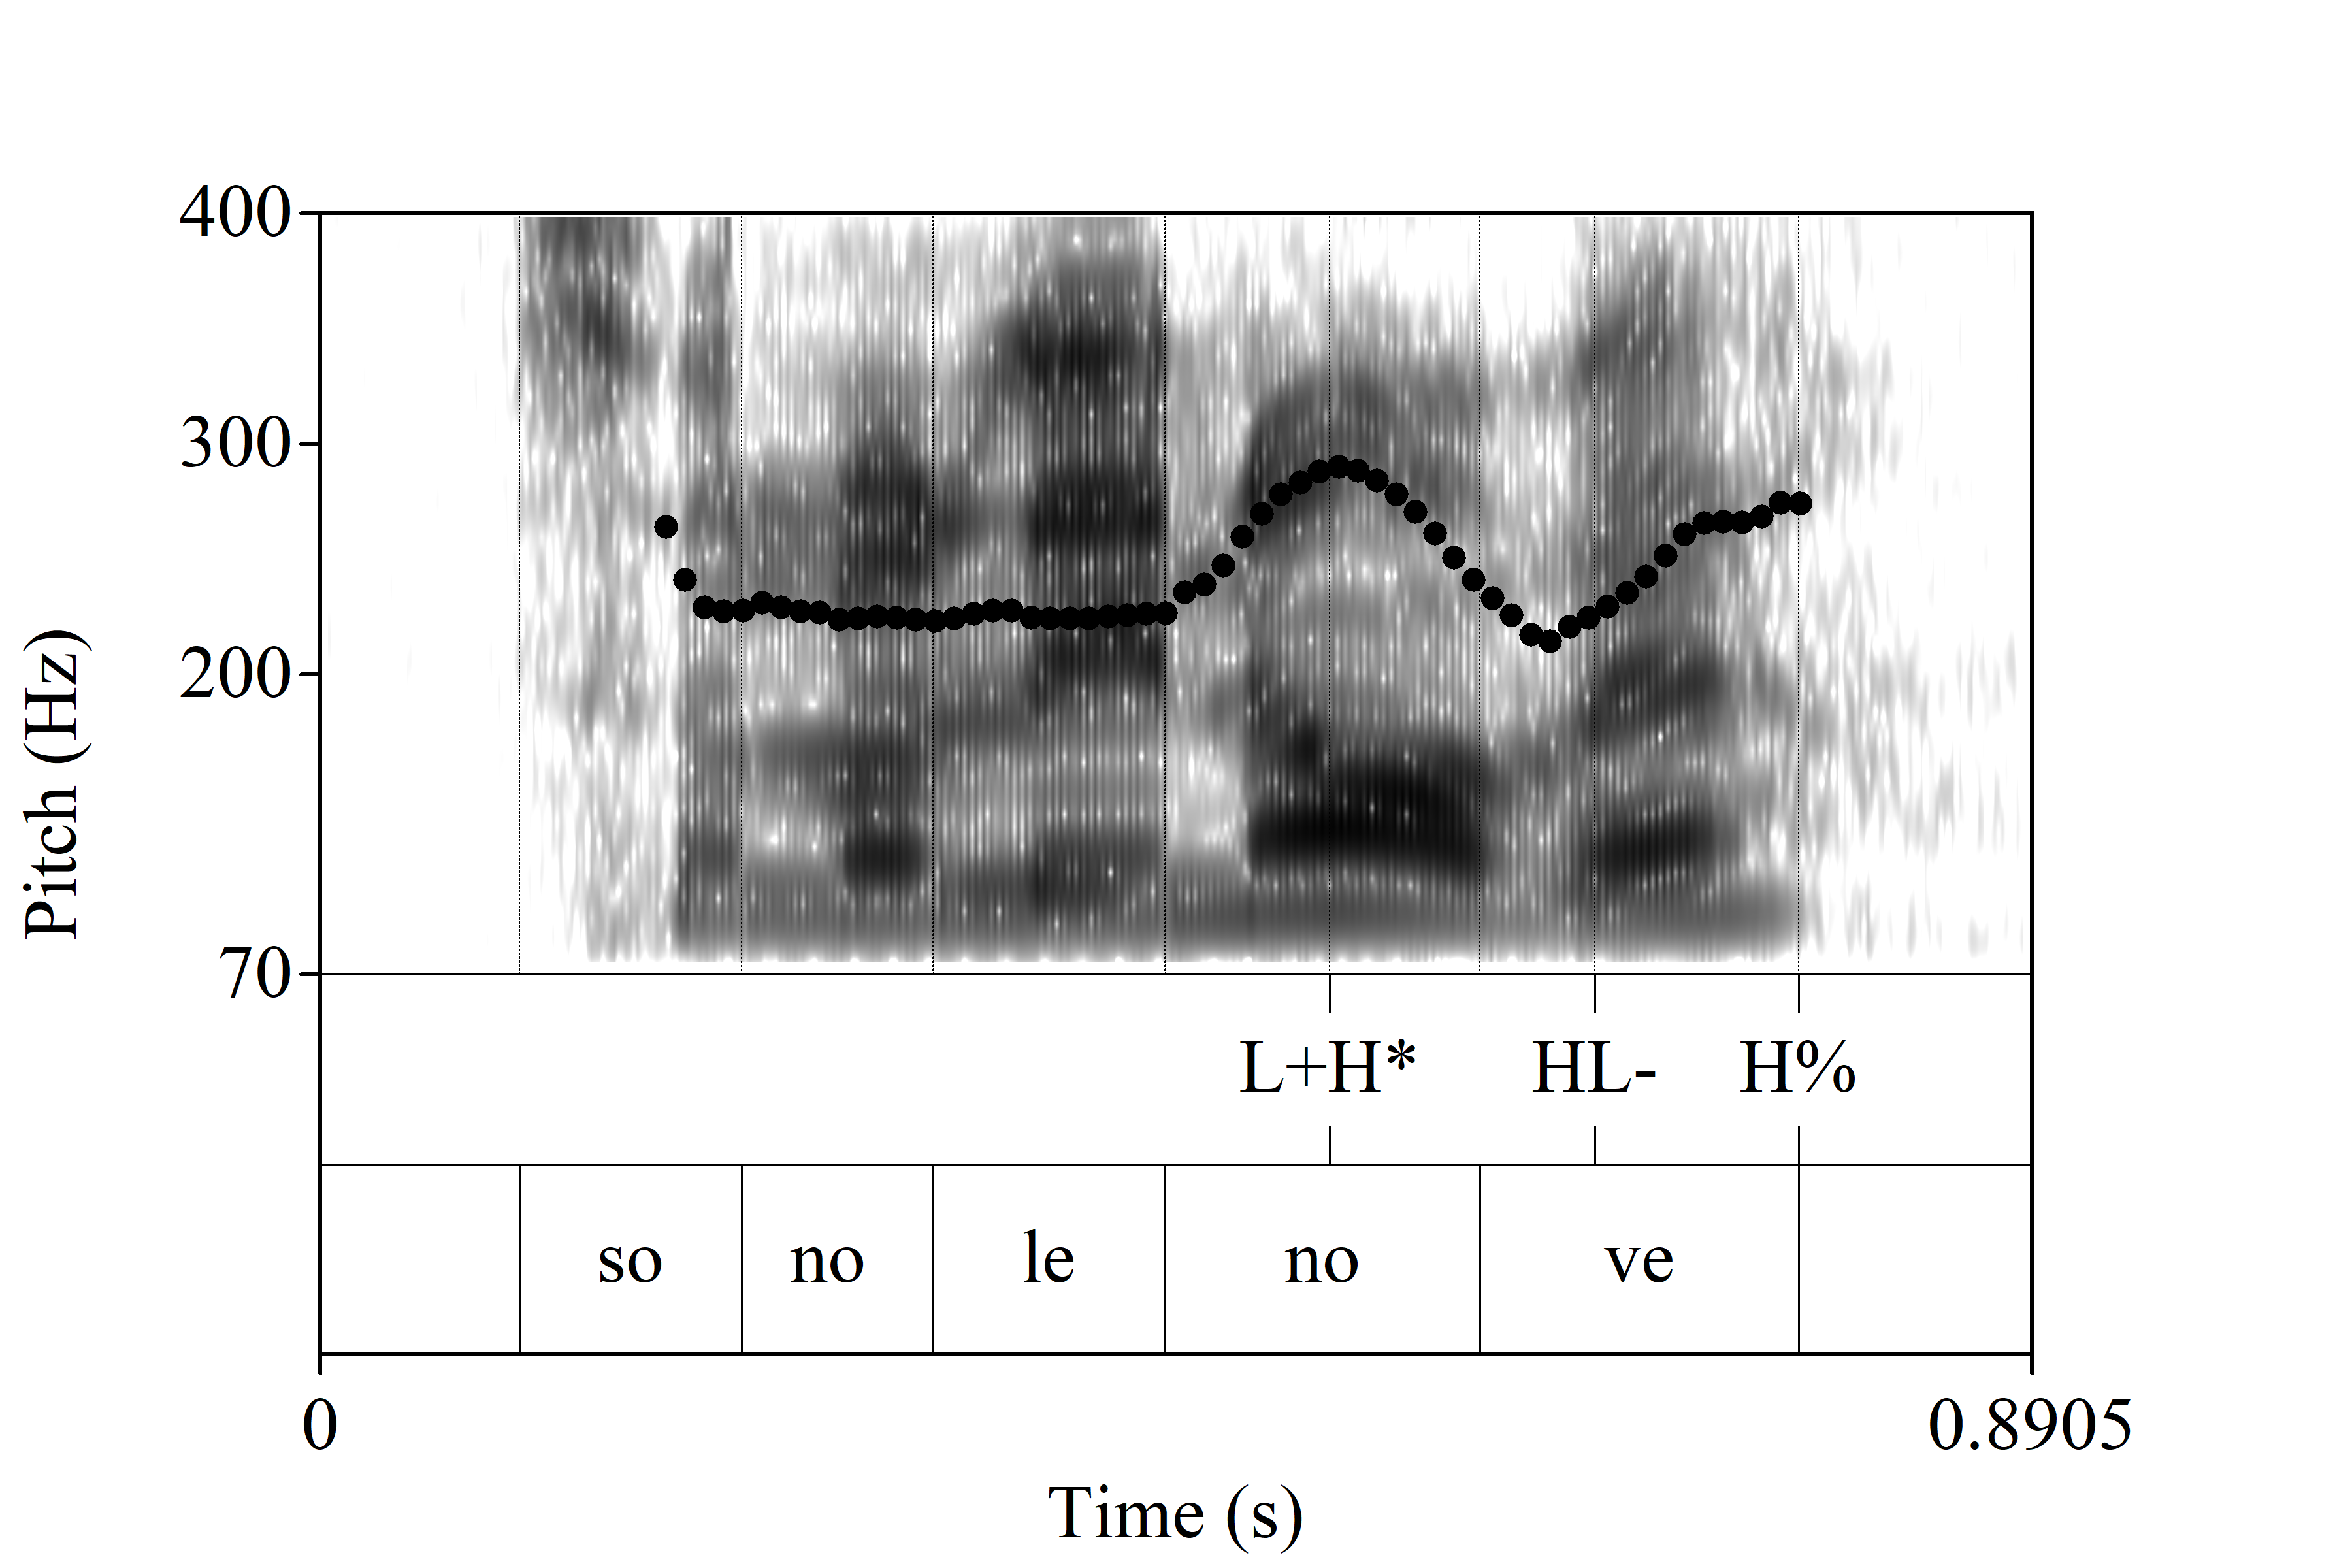
\includegraphics[width=.45\textwidth]{figures/ch10-1a.png}
    }
  \subfigure{
    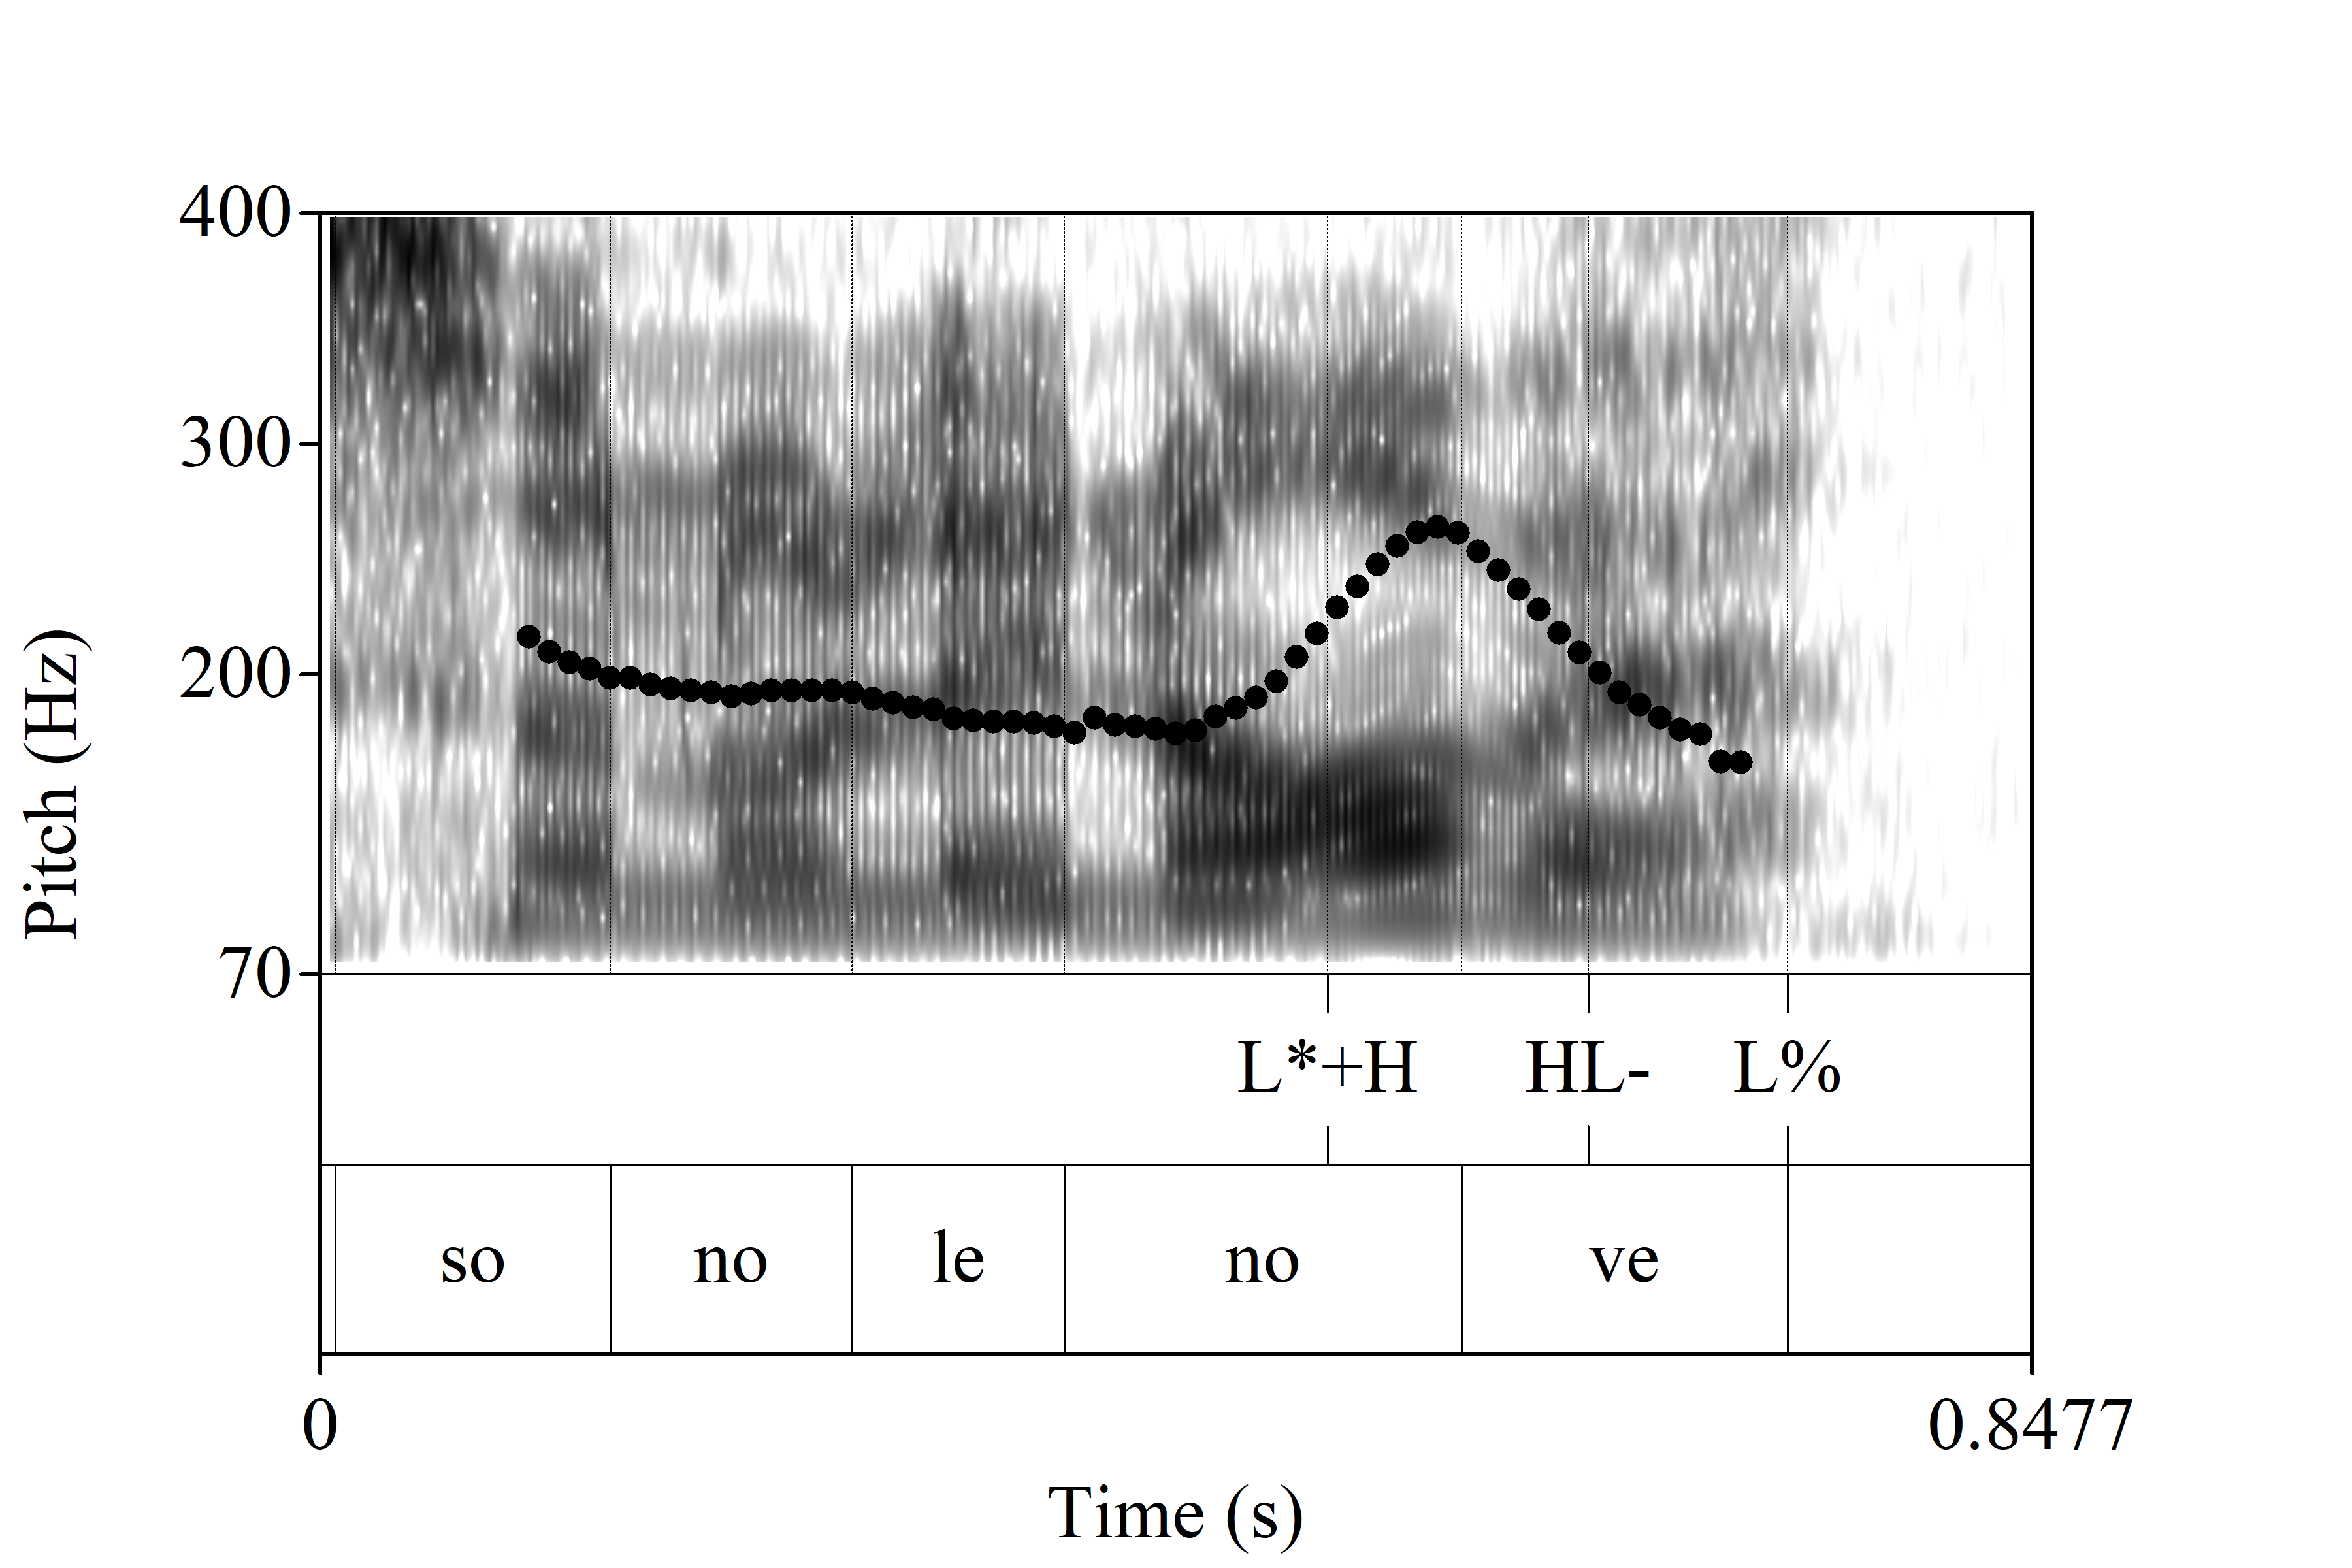
\includegraphics[width=.45\textwidth]{figures/ch10-1b.png}
    }
  \subfigure{
    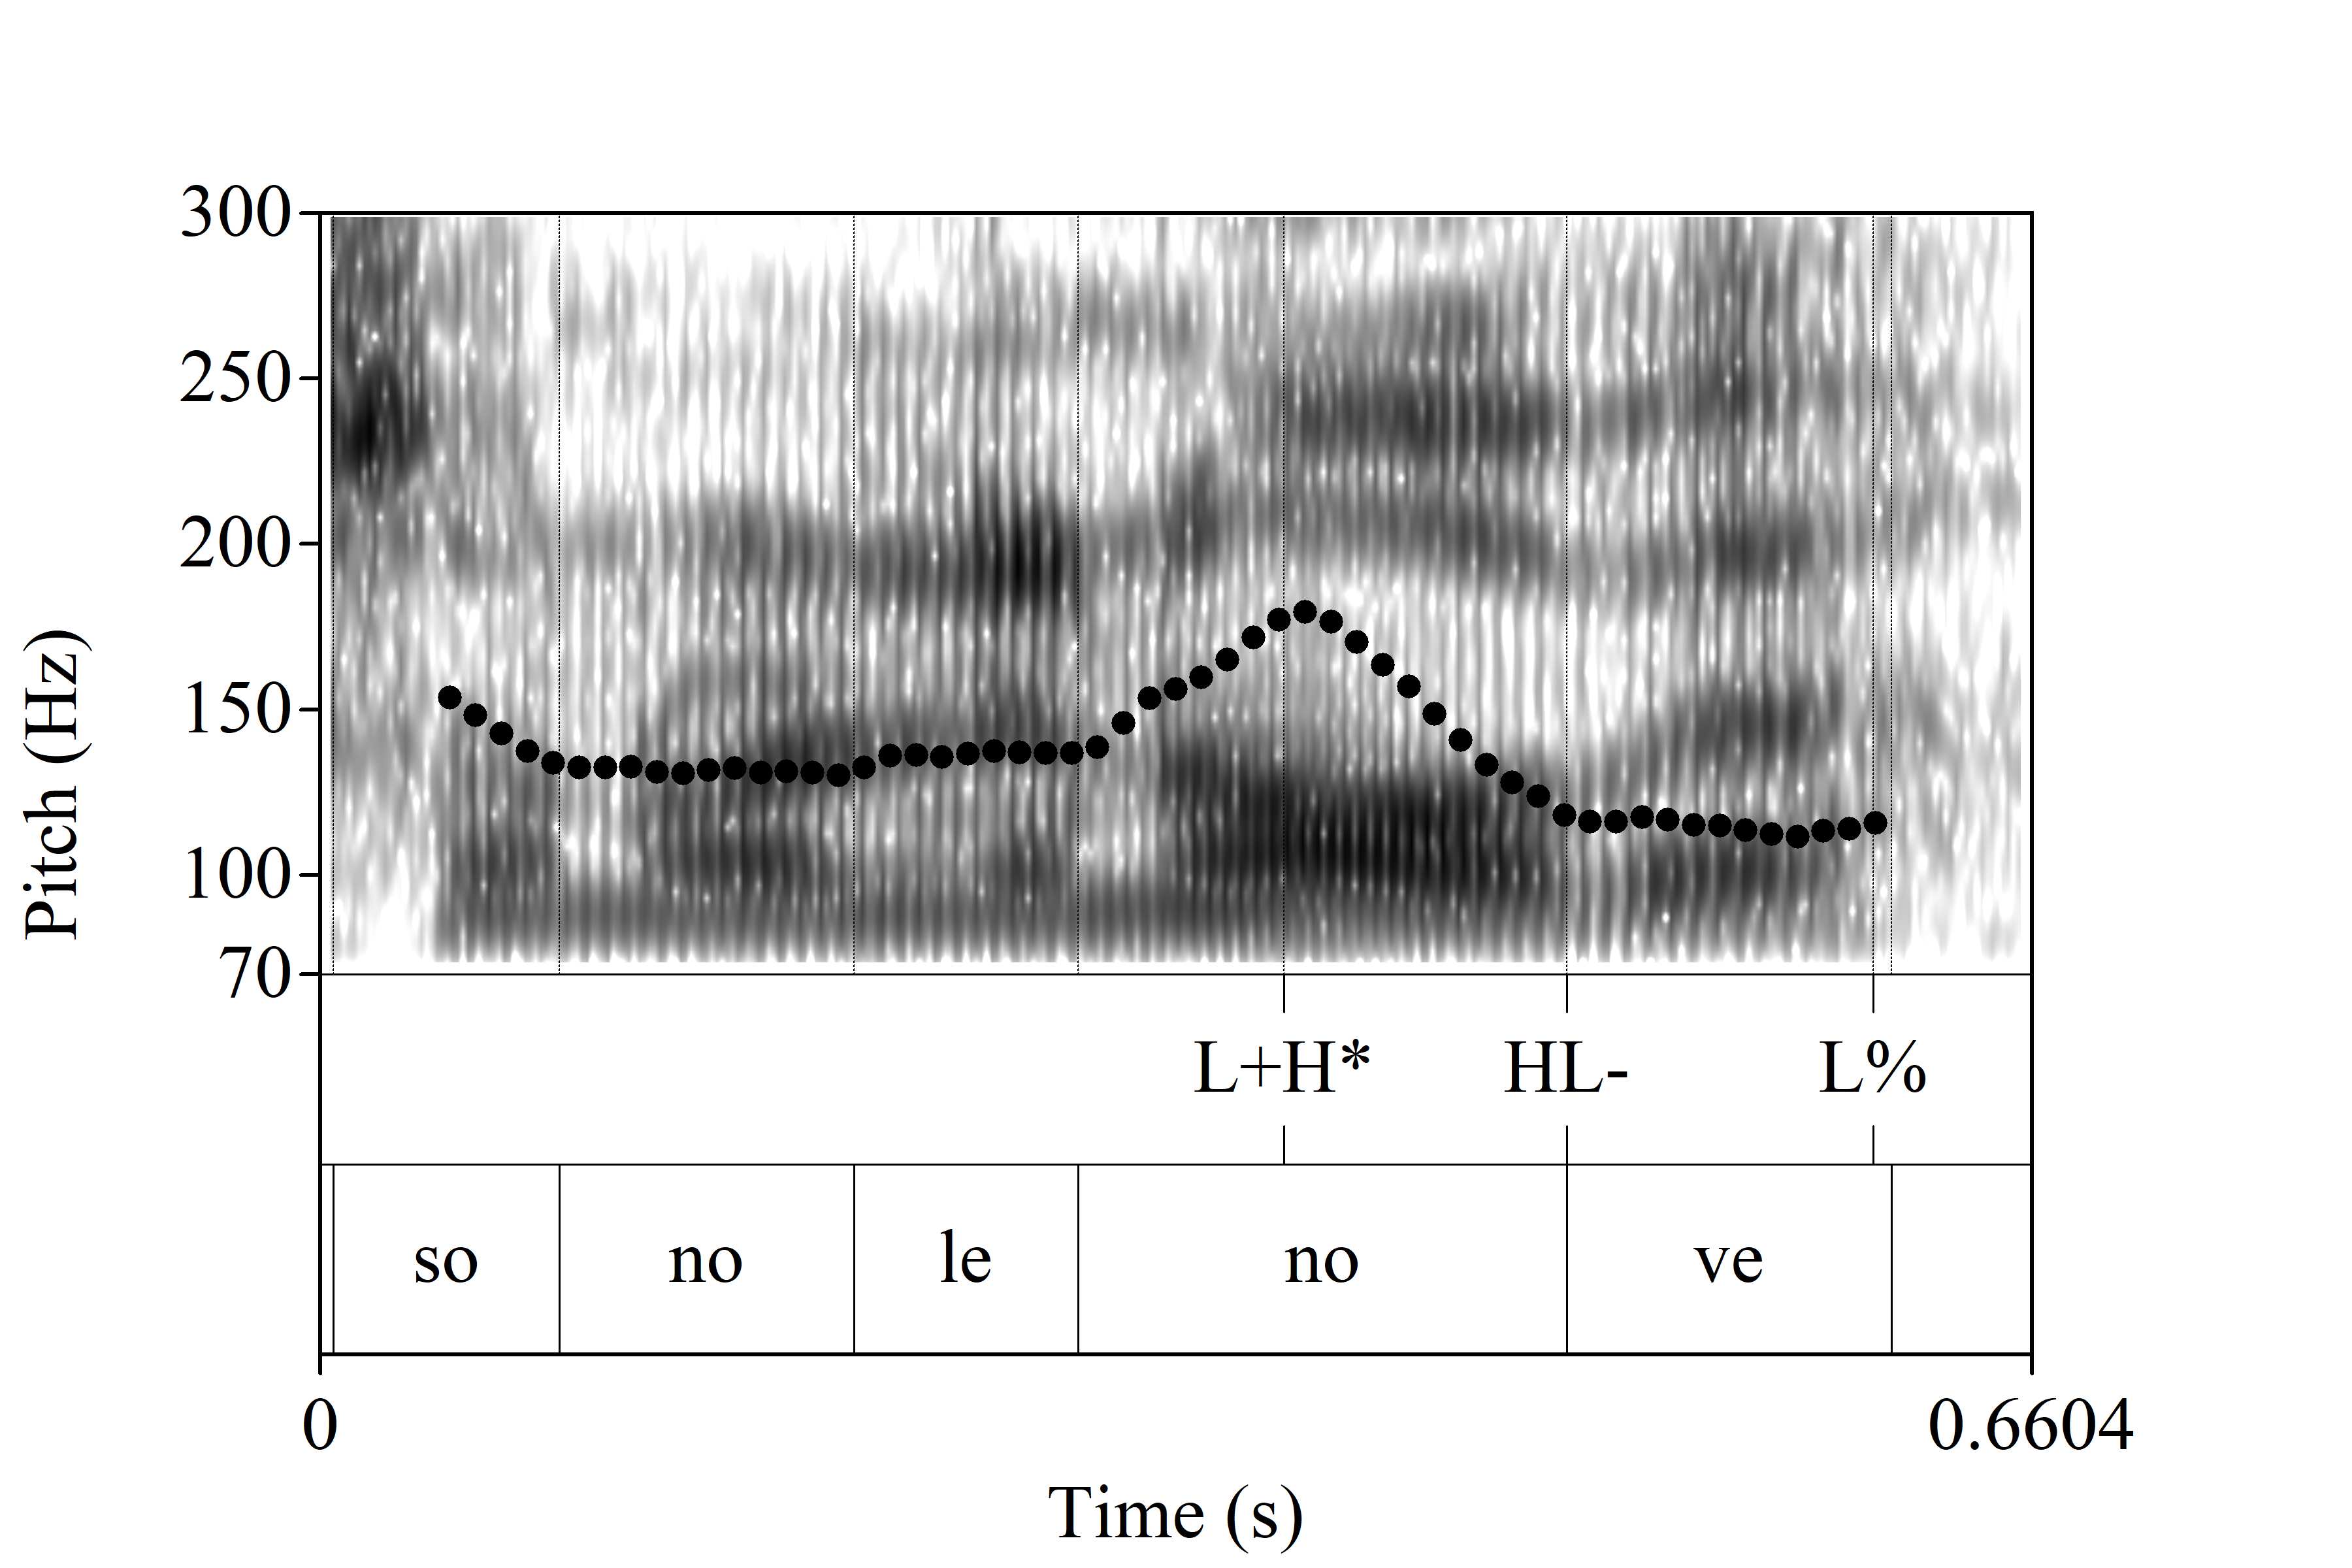
\includegraphics[width=.45\textwidth]{figures/ch10-1c.png}
    }
  \subfigure{
    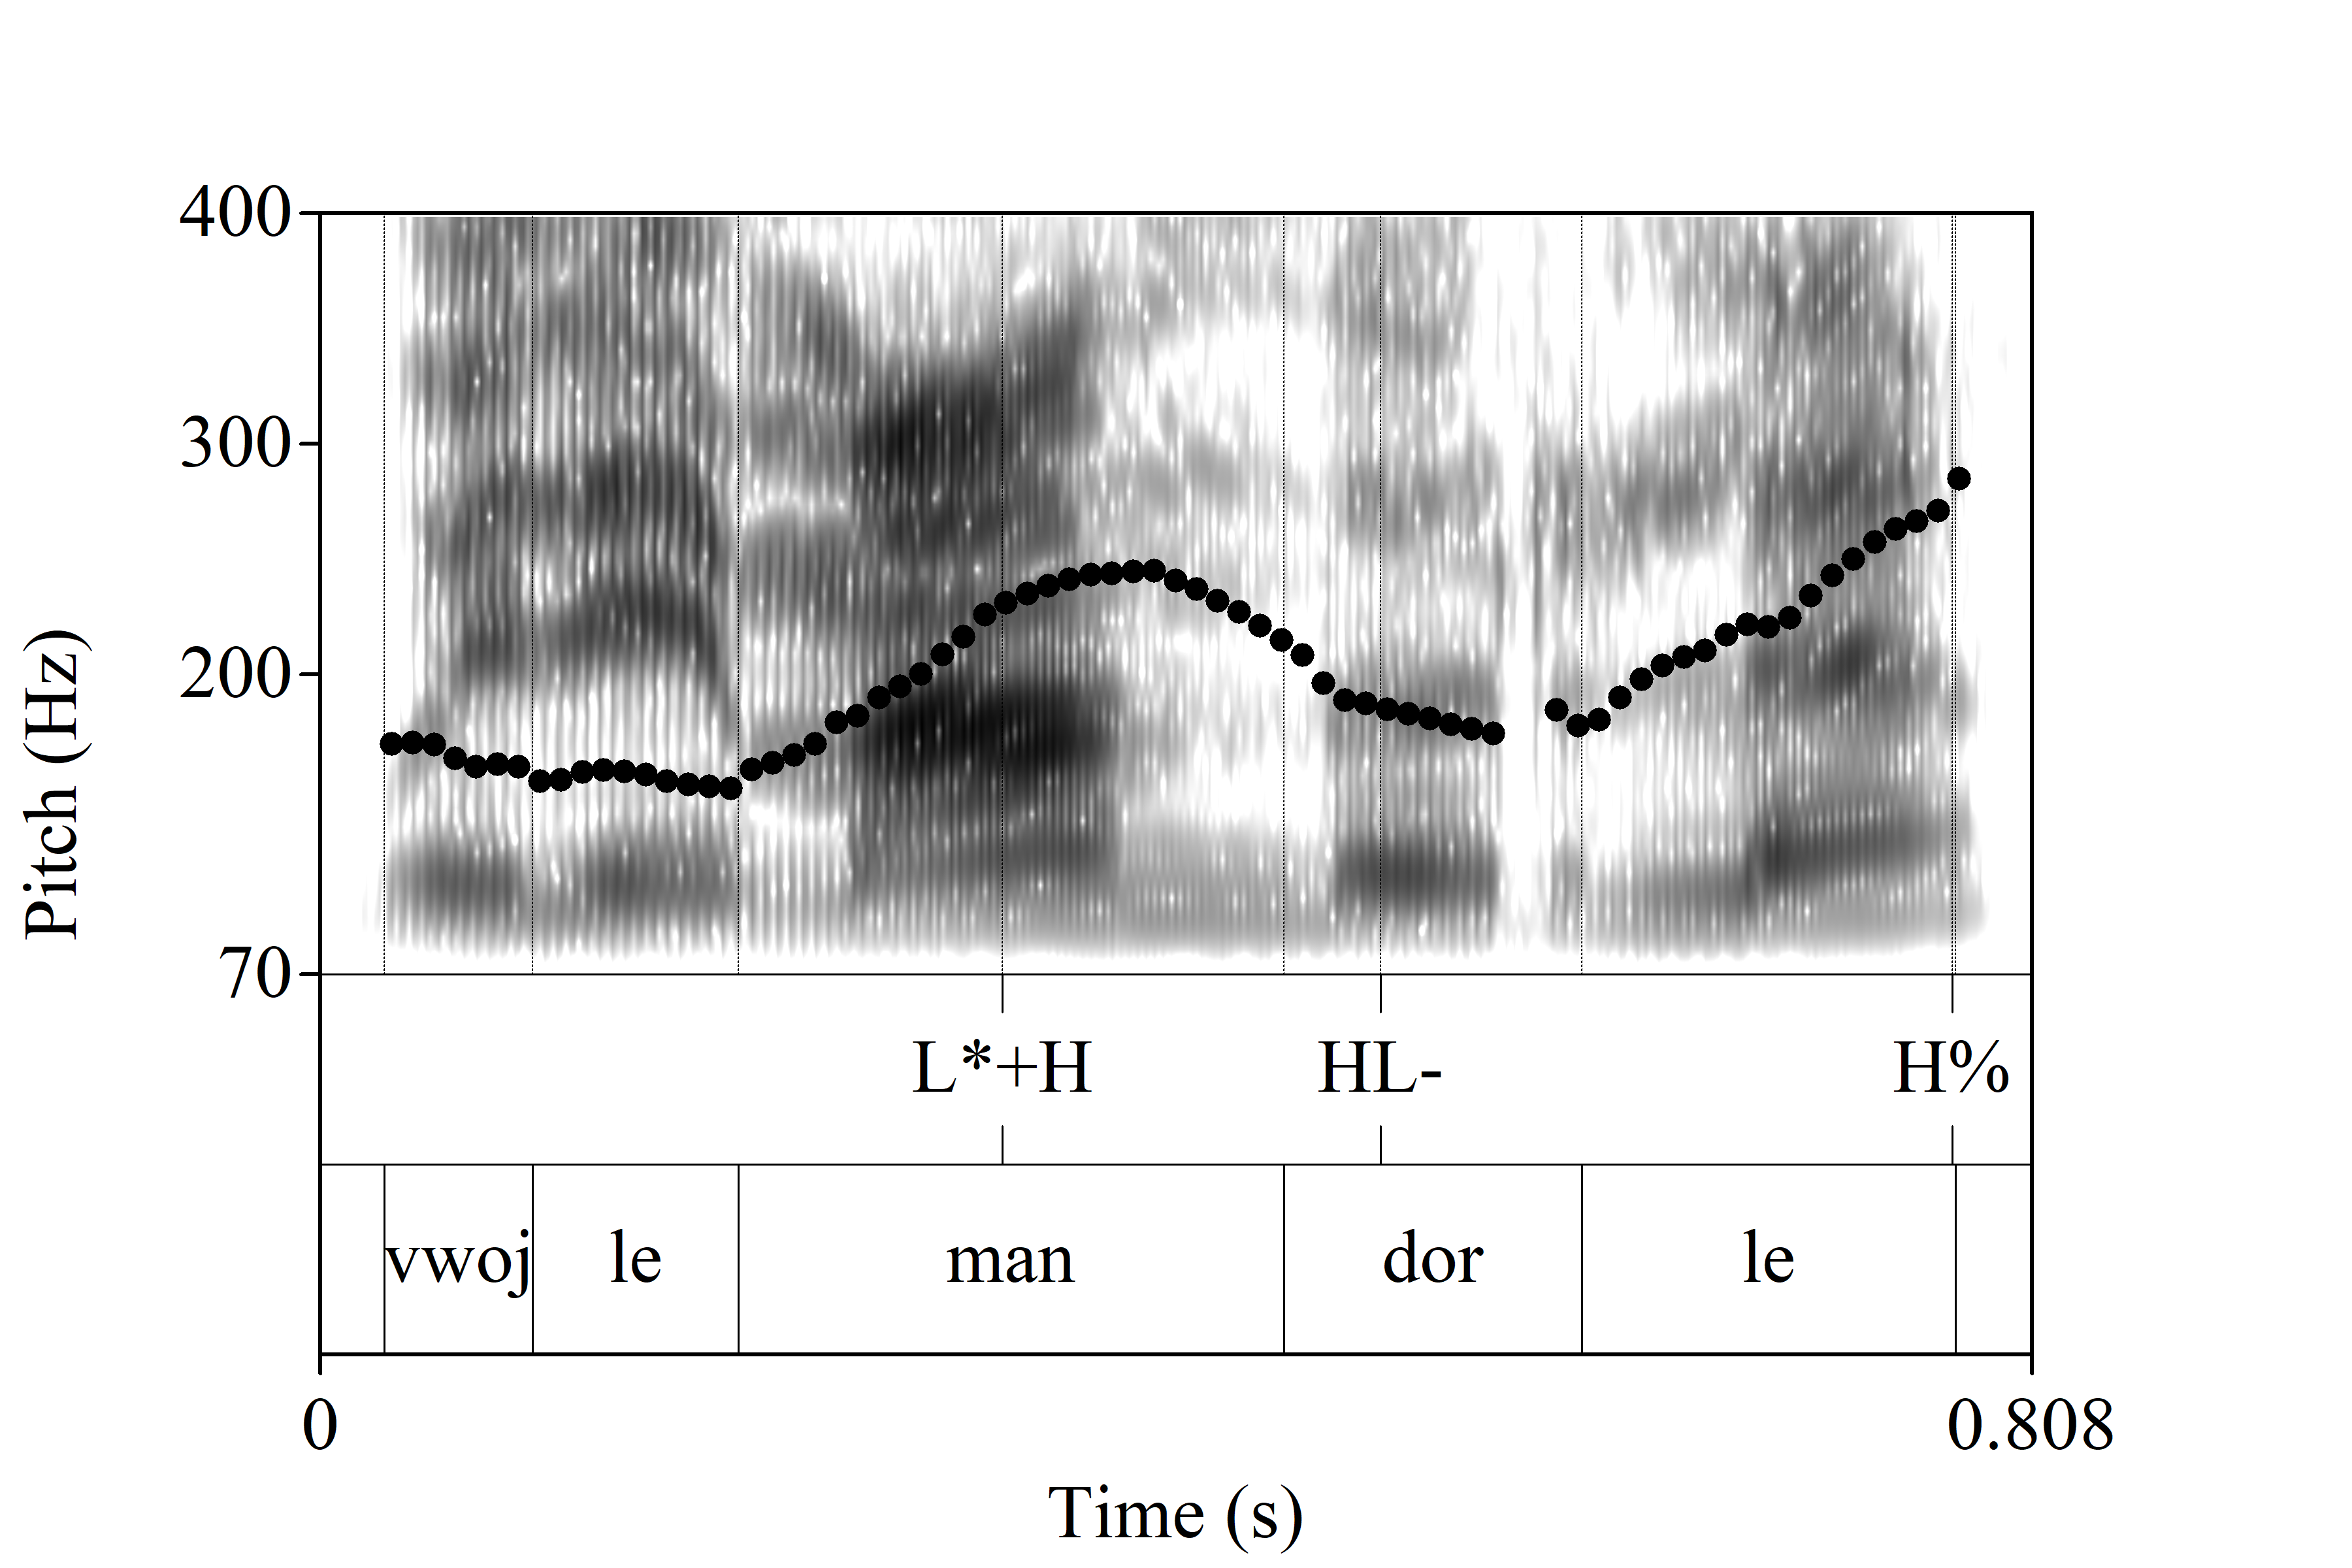
\includegraphics[width=.45\textwidth]{figures/ch10-1d.png}
}
  \caption{Example of yes/no question tunes attested in Salerno Italian by \citep{orrico19}. The figure shows three contours of the utterance \textit{Sono le nove?} 'Is it 9 o' clock?' uttered with a L+H* HL-H\% (top left) L+H* HL-L\% (bottom left) and L*+H HL-L\% (top right) and one contour for the question \textit{Vuoi le mandorle?} 'Do you want the almonds?' uttered with a L*+H HL-H\% (bottom right).}
  \label{fig1}
\end{figure}

Note that polar questions can be expressed with two different nuclear pitch accents, specifically an early-peaked rise analysed as a L+H* (realized as rising-falling movement within the accented syllable) and a late-peaked rise, labelled L*+H (realized as a rise through the syllable nucleus ending at the vowel offset). Both of these accents are combined with either a rising or a falling boundary tone. Crucially, a falling HL- phrase accent between the pitch accent and the boundary tone appears to be a mandatory cue for polar questions. These four nuclear tunes had very different frequencies of occurrence within the data analysed: the L+H* HL-H\% tune was the most frequent one, accounting for more than 50\% of the productions; the least attested was the L*+H HL-L\% tune, with only a 10\% of occurrences, while the L*+H HL-L\% and L+H* HL-L\% tunes were found to account for the remainder of the cases, with roughly equal distributions.

In spite of the differences in distribution, all these tunes represent a choice for SI speakers to express a polar question. The first thing that can be noticed is that in SI, as also reported for other varieties of Italian, a final rise is not a necessary condition for expressing a polar question (\citealt{Fivelaetal15}; see also \citealt{savino2012} for a general account of polar questions). Indeed, contrary to most descriptions of intonation in other languages, rising boundary tones represent only a possibility on the paradigmatic axis, rather than being the primary cue to questionhood. The same status appears to be compatible with the use of pitch accents in nuclear position, with speakers having the possibility of selecting either an L*+H or an L+H*.

Note that literature on Italian intonation has assigned nuclear pitch accents, rather than boundary tones, a crucial importance in the definition of an utterance as a polar question. \citet{griceetal2005}, building on previous studies \citep[e.g. ][]{grice1995, savino1997, dimperio2002}, put forward the idea that, especially for southern varieties, the phonological identity of a nuclear pitch accent is the main cue for questionhood. Later research has challenged this idea: other cues beside nuclear pitch accents have been found to be responsible for sentence modality identification – e.g. prenuclear region \citep{petrone2011} or temporal patterns \citep{cangemind2015}. Nevertheless, the disambiguation provided by pitch accent choice, as far as the question vs. statement opposition is concerned, is strong in several varieties. The role of boundaries, on the contrary, has often been linked to speech style and/or attributed to the unnaturalness of the experimental condition during data collection \citep{savino2012, cangemigrice2016} rather than representing a specific pragmatic choice of the speaker. Nevertheless, in the specific case of SI, phrase boundaries, as well as pitch accents, appear to be sufficient cues for expressing a polar question and are linked to the expression of specific pragmatic meanings (e.g., \citealt{orrico19} did not observe any distributional differences manipulating the naturalness of the task employed, i.e. Discourse Completion vs. Reading Task).

Analyses of production data show that nuclear accent position within a sentence might also be involved in the expression of sub-meanings within a polar question. Note that within the intonational phonology of Italian, a nuclear pitch accent does not have to be the rightmost accent within an utterance. Rather, a nuclear pitch accent can be placed early in the sentence, being followed by a post-nuclear accent, typically downstepped \citep{griceetal2005, dImperioetal2020}. Additionally, in case of complex accented constituents, the rise-fall movement can be stretched over the whole constituent, creating a high plateau (hat pattern). In these cases, the accentual rise is moved leftward and placed on the first stressed syllable of the constituent, while the HL- phrase accent is placed on the last stressed syllable of the same constituent. This pattern, when found in polar questions, was analysed in Neapolitan Italian by \citet{dimperio2002} as a L*+H H(*)L-L\%, with the parenthesized star (*) indicating that the phrase accent is secondarily associated with a stressed syllable \citep[see also][]{prietoetal2005}. A similar pattern is attested in SI, as shown in \figref{fig2}.

\begin{figure}
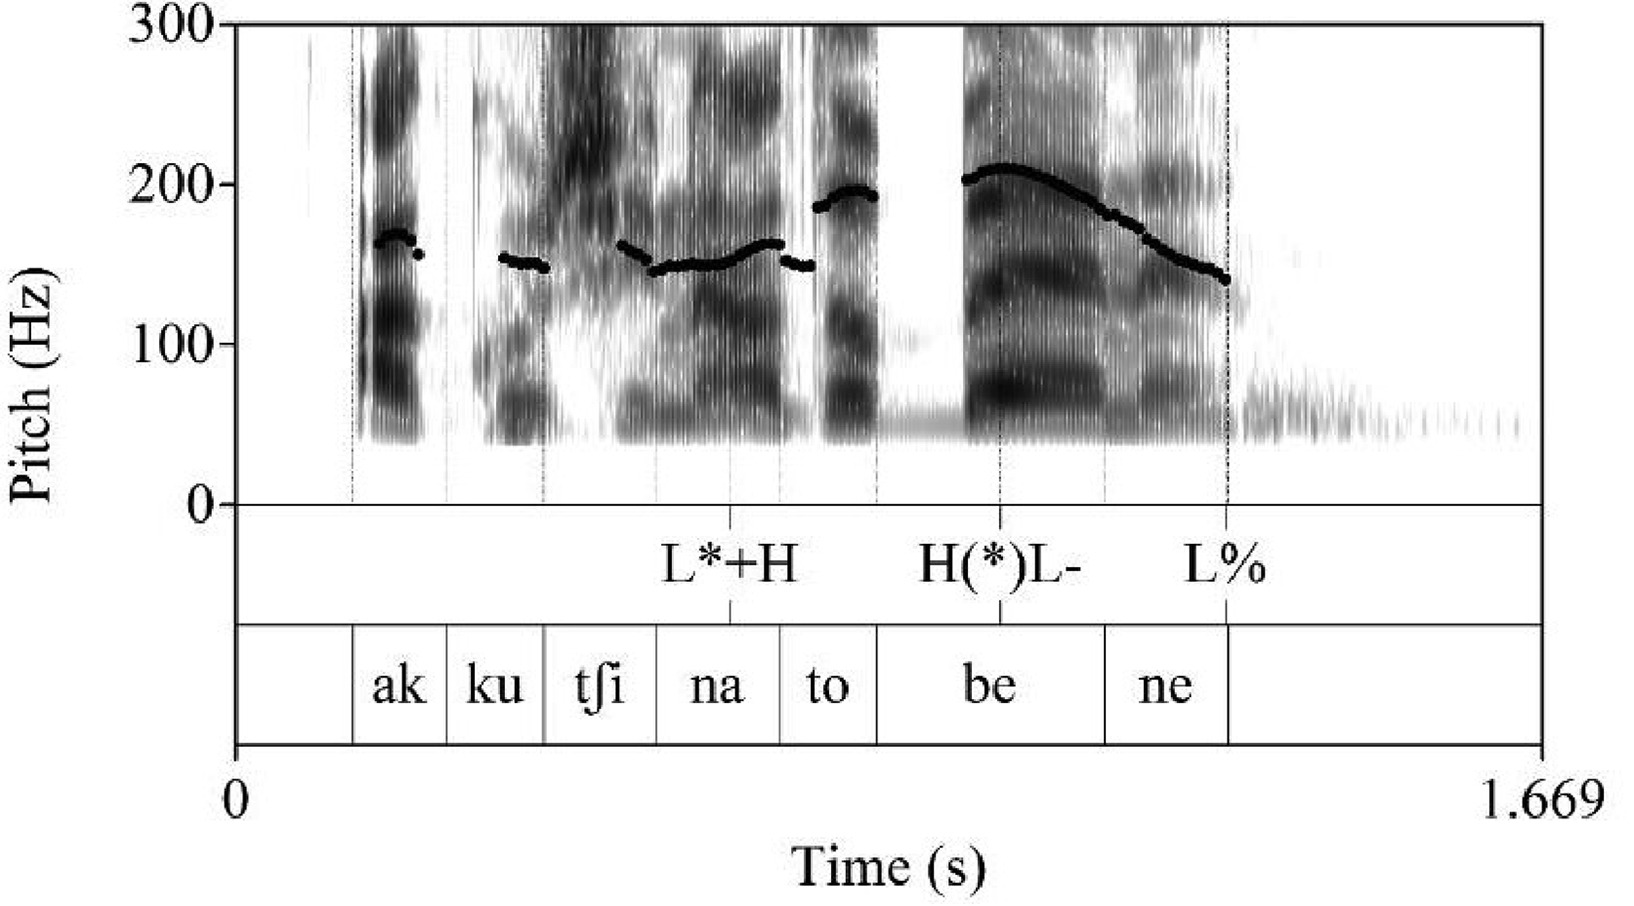
\includegraphics[scale=1]{figures/ch10-2.jpg}
\caption{F0 contour for the question utterance \textit{Ha cucinato bene?} (Did s/he cook well?) uttered with a L*+H H(*)L-L\% tune.}
\label{fig2}
\end{figure}

\newpage
Recent studies investigating the issue on both the production and perception sides have found that both tune choice (pitch accent and boundary type) and nuclear accent placement are involved in the conveyance of the epistemic position of the speaker towards the utterance. Despite data from production, showing high levels of inter-speaker variability, some patterns were found to correlate with specific pragmatic conditions. For example, the analysis of distribution reported in \citet{orrico19} shows that a L+H* HL-L\% contour is mainly employed in the counter-expectation condition (i.e., the speaker is rejecting some information provided by the addressee). As for perception, an experiment recently reported in \citet{orrico2022} was designed with the aim of testing whether and how phonologically different tunes could be interpreted by SI listeners as mapping onto different degrees of speaker certainty towards the expected answer. The tunes investigated were the rise-fall-rise tune with the early-peaked pitch accent (L+H* HL-H\%) and the two rise falls, differentiated on the basis of the pitch accent (i.e. L*+H HL-L\% and L+H* HL-L\%). Additionally, the L*+H H(*)L-L\% tune was included in the experimental design to test whether the pitch accent placement could play a role in the conveyance of these meanings. 45 SI listeners took part in the experiment. They were asked to listen to questions out of context and to rate them by assigning a score (from 0 to 100) according to the degree of perceived certainty of the speaker for a specific answer to the question. Results show that specific cues within question tunes are exploited by SI listeners to extract bias information. Specifically, the L+H* HL-H\% tune was found to be rated significantly higher in speaker certainty than L+H* HL-H\%, while the L*+H HL-L\% was globally rated the lowest in certainty score. Additionally, the tune with a nuclear pitch accent placed earlier in the utterance (L*+H H(*)L-L\%) received the highest certainty score.

Finally, a further element of variation across question tunes is the pitch excursion within the pitch accent. In fact, data from Salerno Italian show that questions can have at least two different distributions as far as the excursion of the pitch accent in nuclear position is concerned, as shown in \figref{fig3}.

\begin{figure}
  \subfigure{
      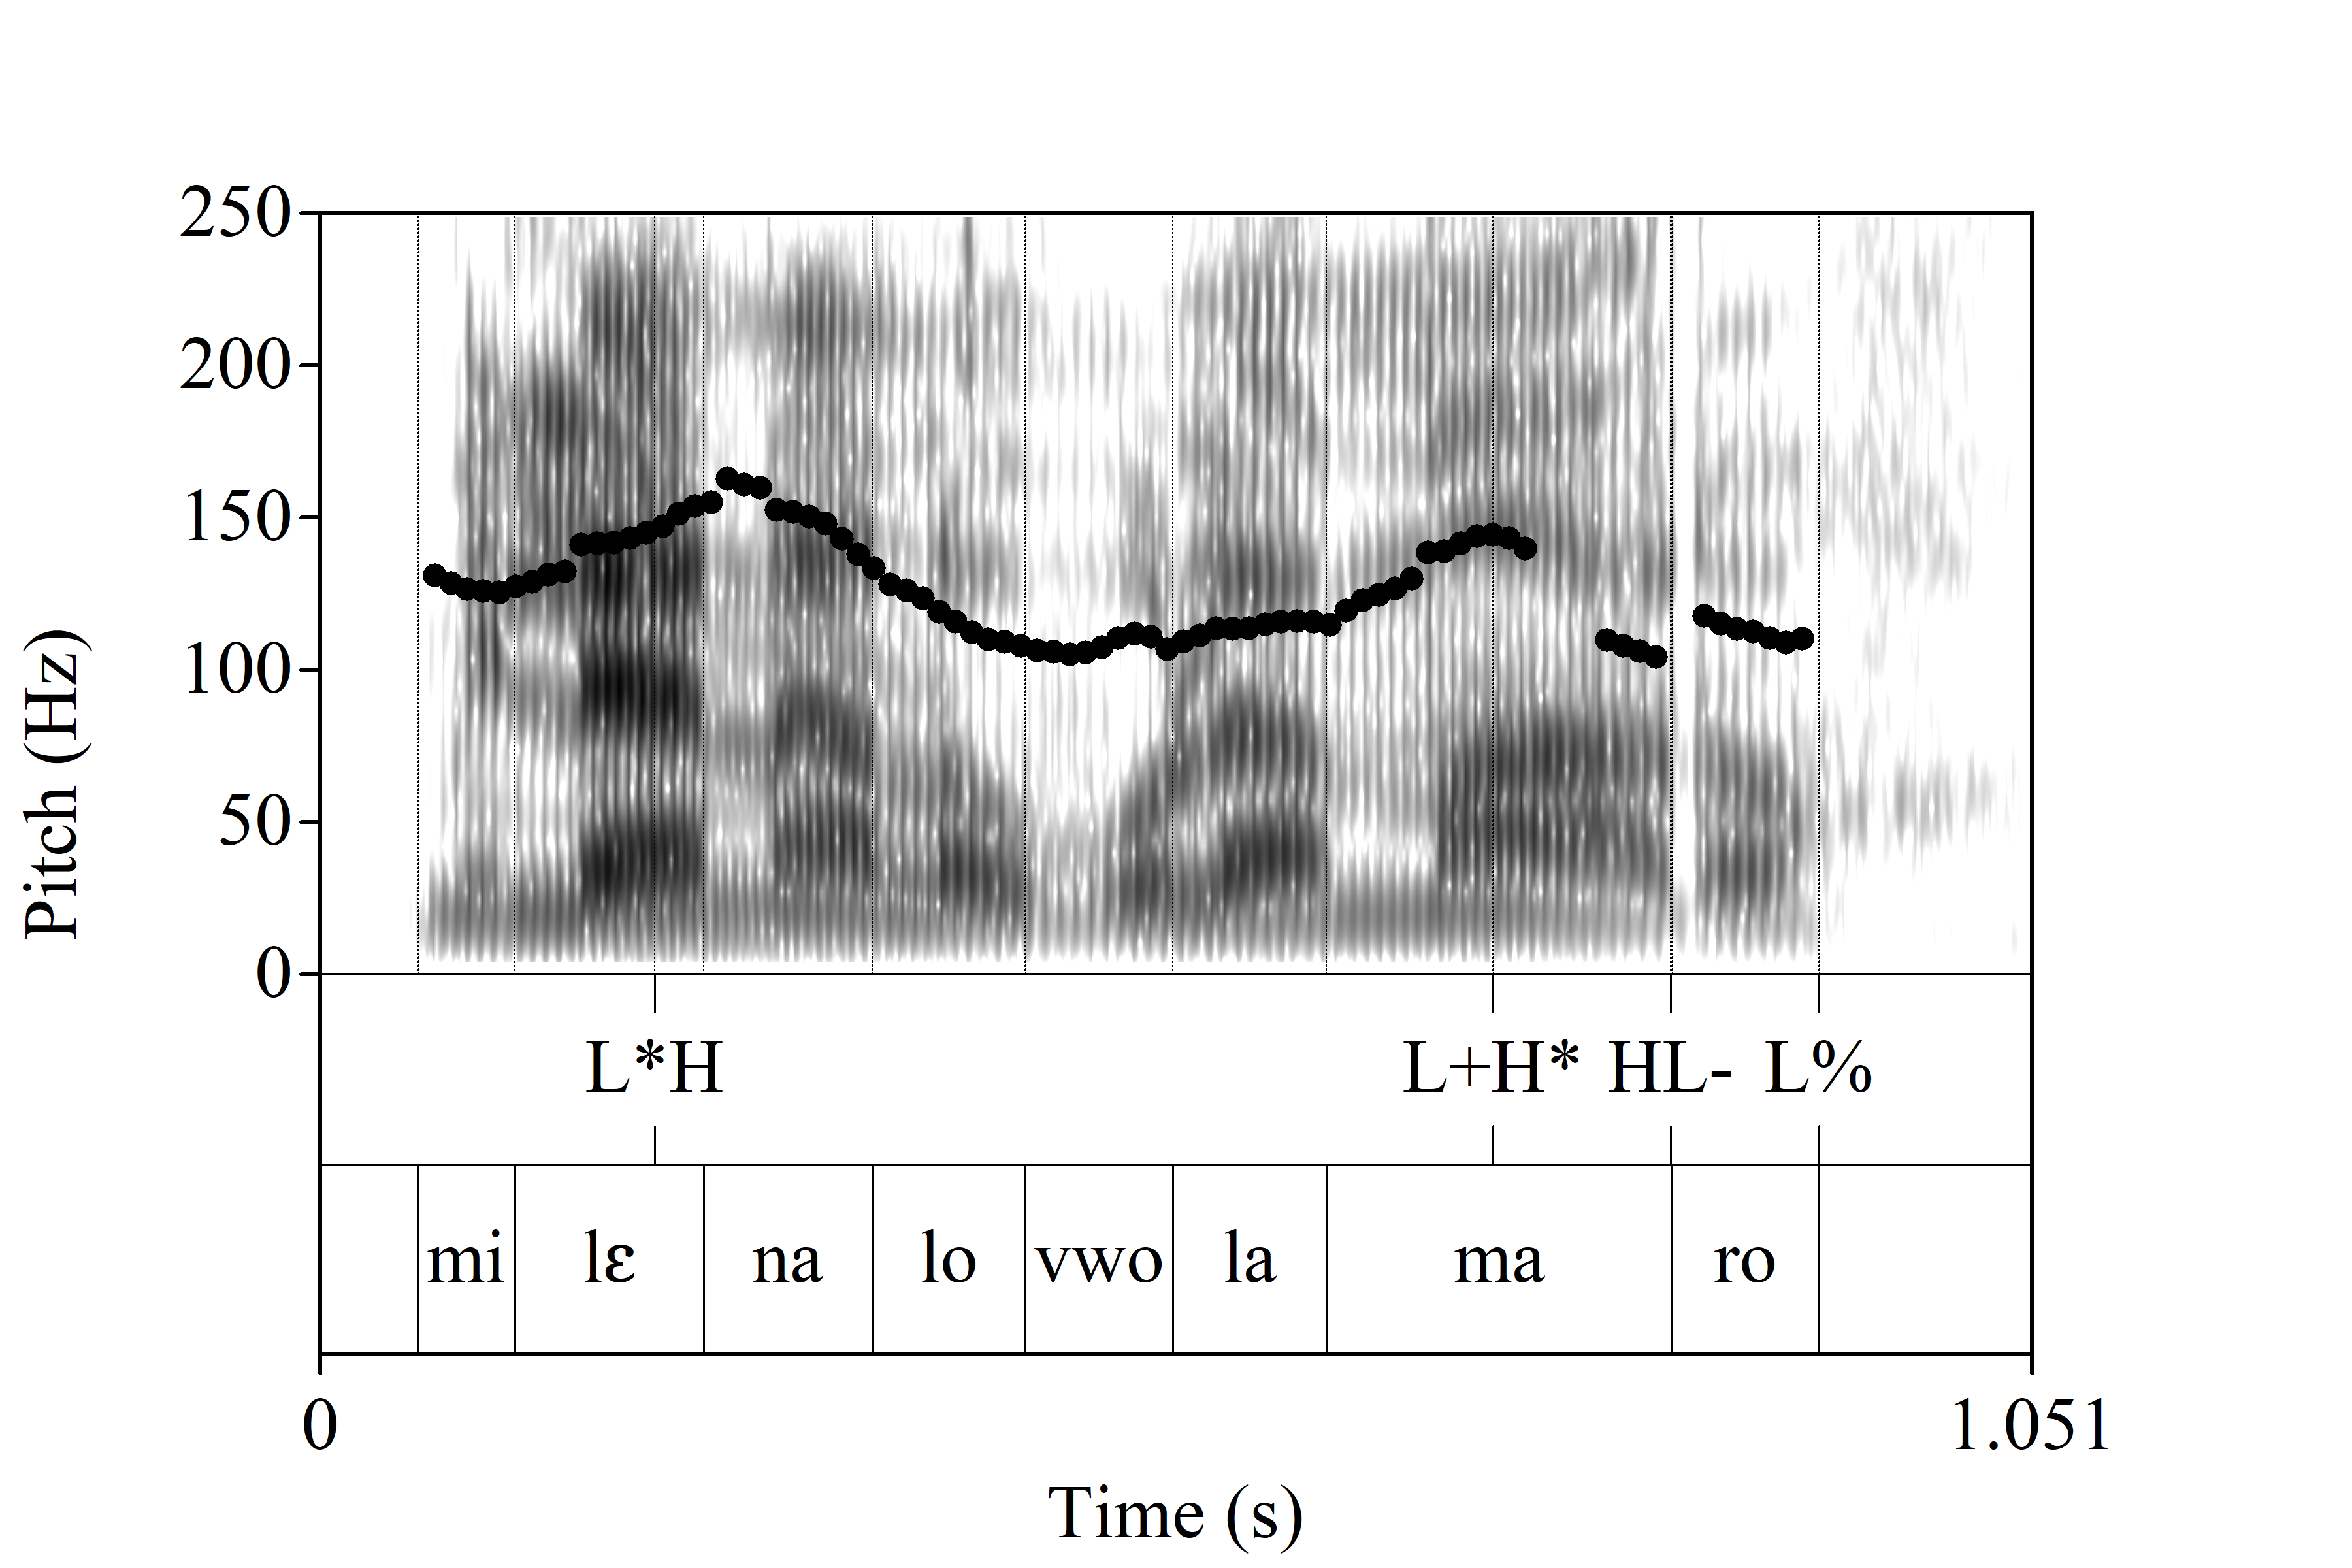
\includegraphics[width=.45\textwidth]{figures/ch10-3a.png}
    }
  \subfigure{
    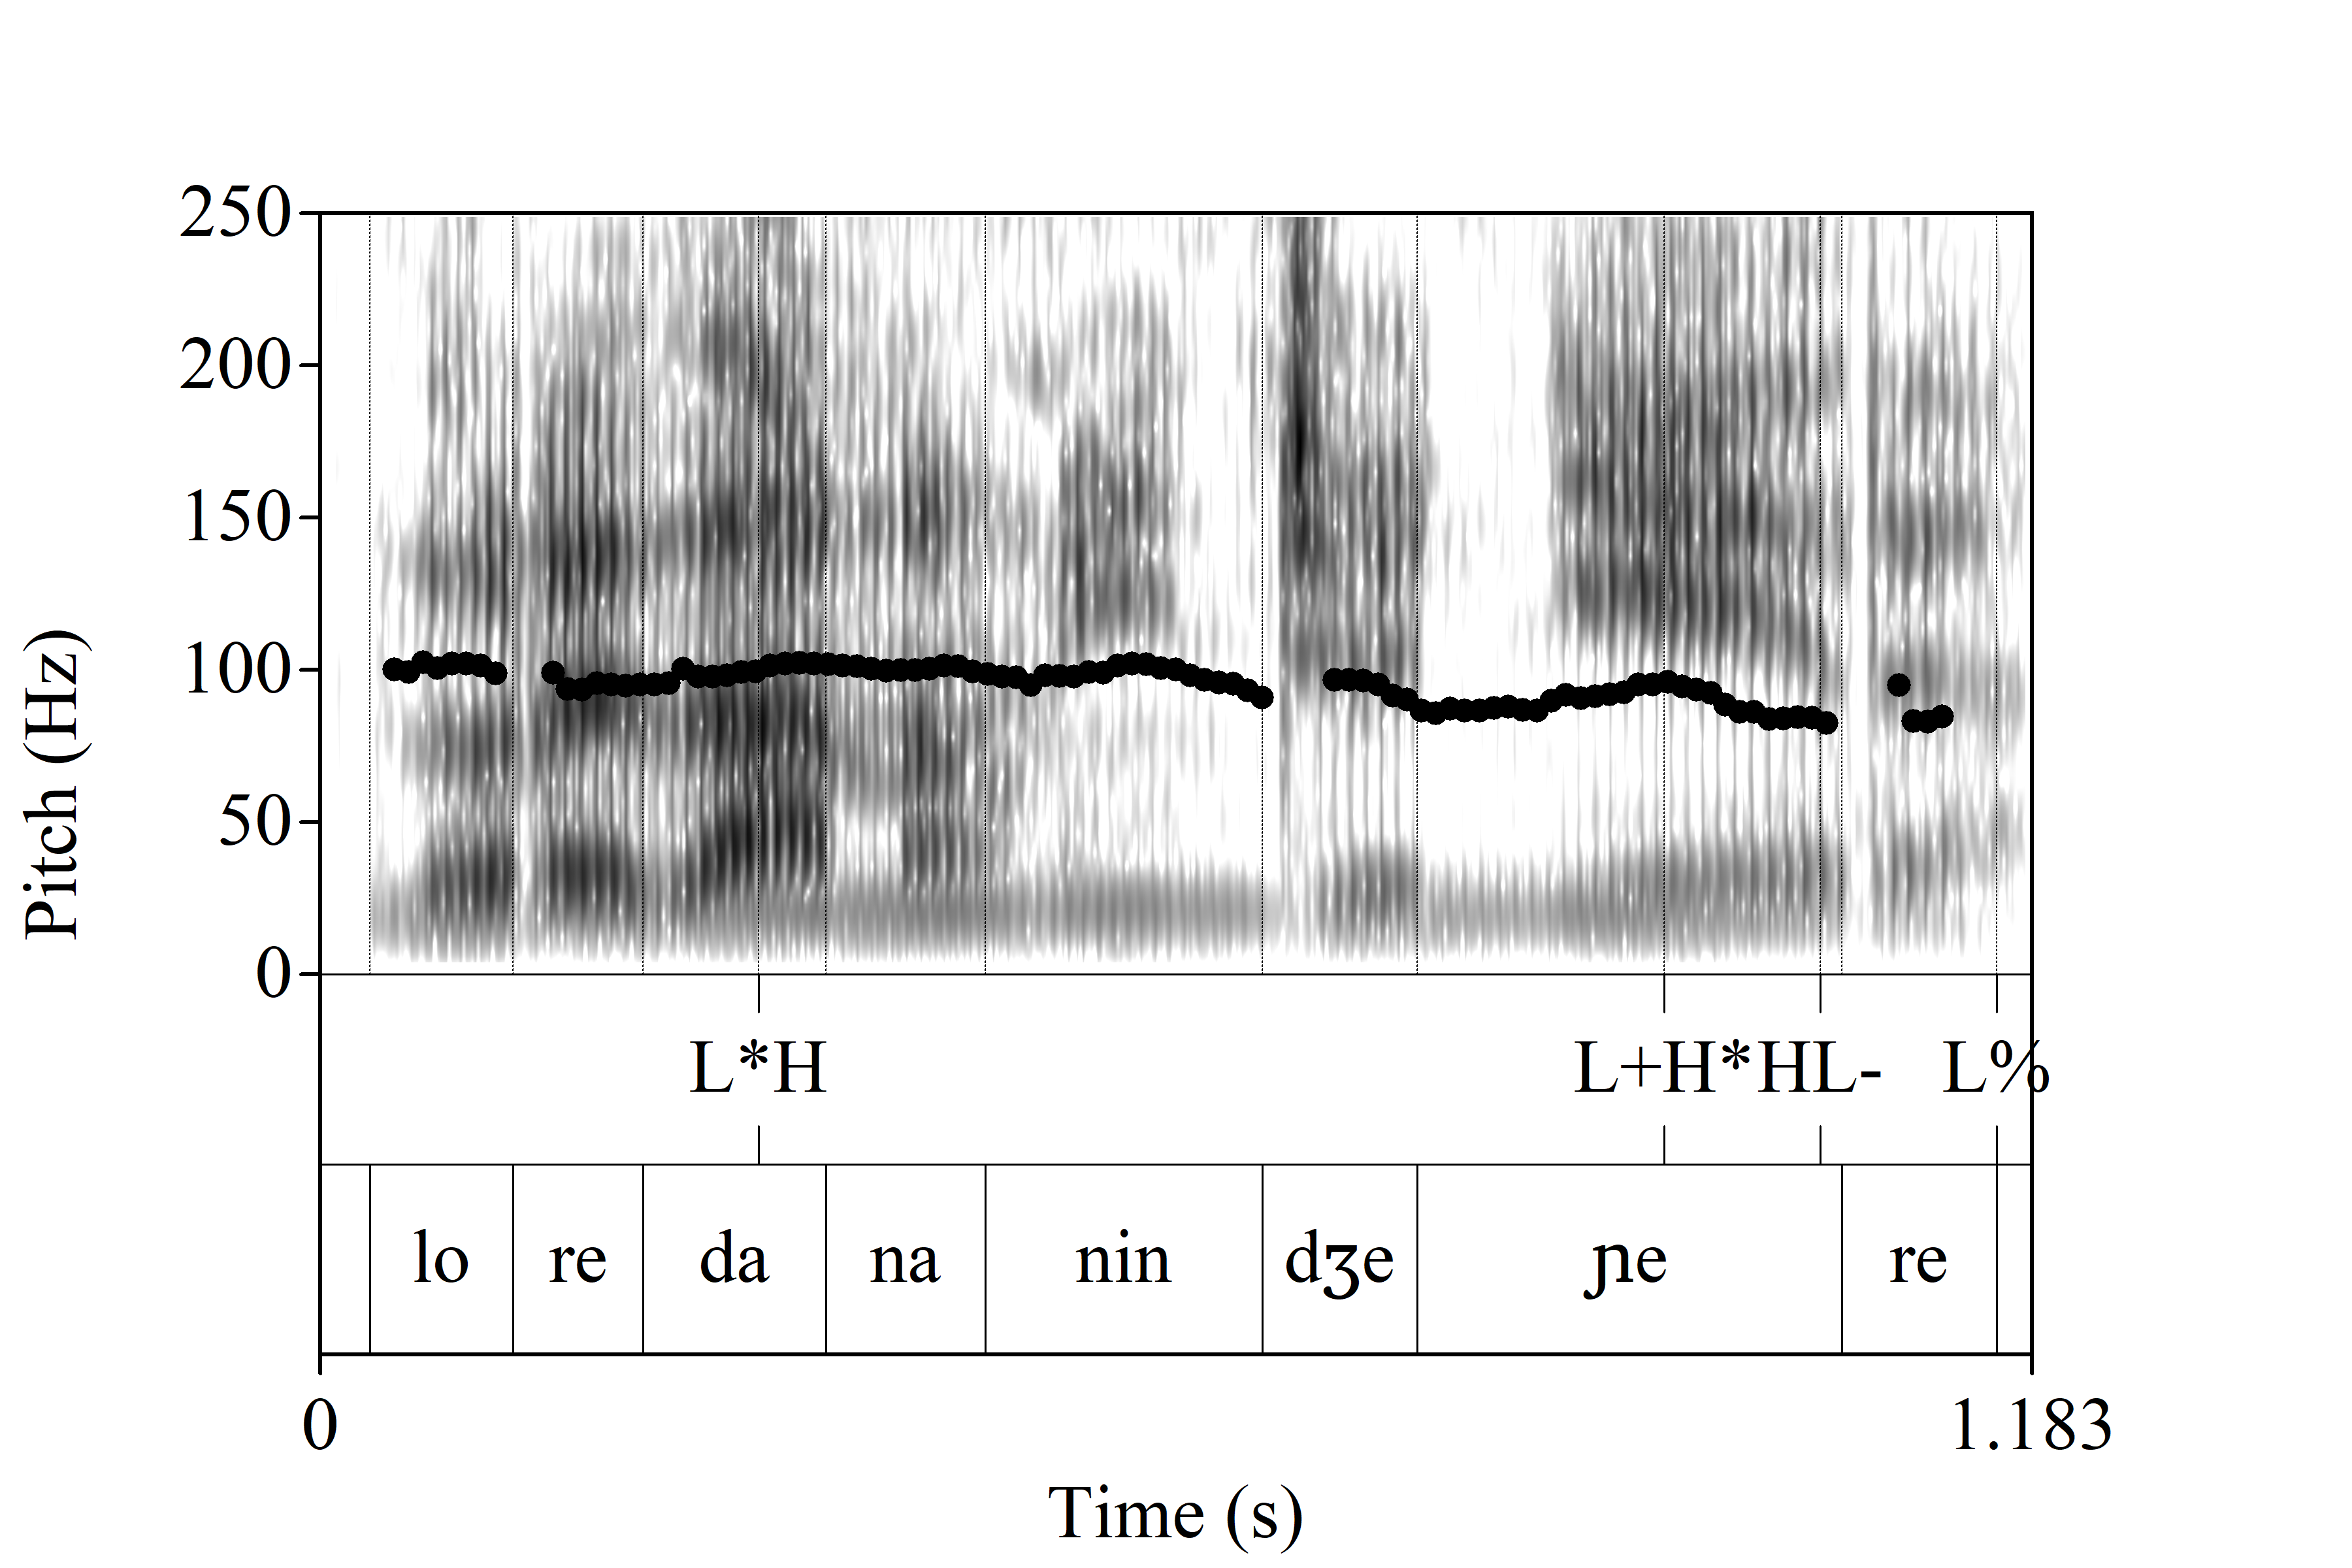
\includegraphics[width=.45\textwidth]{figures/ch10-3b.png}
    }
  \caption{Examples of L+H* with different span values. The figure shows the question utterances \textit{Milena lo vuole amaro?} (Does Milena take it [coffee] black?), on the left, and \textit{Loredana un ingegnere?} (Loredana an engineer?), on the right, uttered by the same male speaker but with a narrower pitch span \citep[adapted from][]{orrico19}.}
  \label{fig3}
\end{figure}

In both examples reported in \figref{fig3}, the nuclear pitch accent produced by the speaker is an early rise (L+H*), though with different pitch span values correlating with specific pragmatic information of the context they were uttered in. More specifically, \citet{orrico19} reported that instances of L+H* nuclear accents with a narrower pitch span were typically employed to encode counter-expectational questions, i.e., when the speaker is conveying his/her incredulity towards the information contained in the question.

A parallel investigation was conducted to perceptually test the role of pitch span within the nuclear region, as reported in \citet{Orrico+2020}. The experimental setting included a collection of the same judgment as in \citet{orrico2022}, that is the assignment of certainty scores by SI listeners, though the manipulated variable was pitch span. 45 participants took part in the experiment; they were asked to rate a set of 18 experimental stimuli, which were artificially created by manipulating the height of the L+H* nuclear accent into three different steps and the height of the boundary tone in six different height steps. Results show (\figref{fig4}) that the wider the span in both pitch accent and boundary tone, the higher the certainty score assigned to the tune. However, while for pitch accent the three different span levels were rated as all conveying a different degree of speaker certainty, the same was not found for boundary tones, given that only the lowest two steps were classified as conveying a significantly different score. In other words, while boundary tones were found to have a categorical effect on the perceived bias of a polar question (corresponding to the two phonological L\% and H\% boundaries), different span levels within pitch accent were found to gradually map onto the pragmatic level.

\begin{figure}
  \subfigure{
      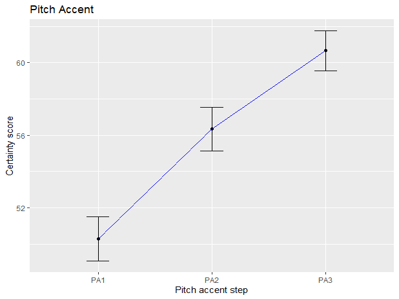
\includegraphics[width=0.45\textwidth]{figures/ch10-4a.png}
}
\subfigure{
    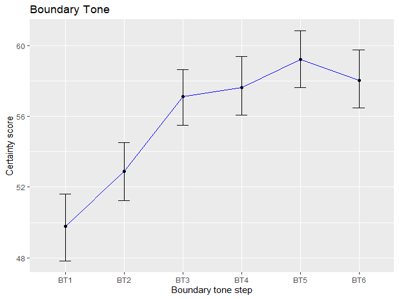
\includegraphics[width=0.45\textwidth]{figures/ch10-4b.png}
}
  \caption{Certainty score assigned to different span values of the L+H* pitch accent (left) and boundary tones (right) \citep{Orrico+2020}.}
  \label{fig4}
\end{figure}

\subsection{French}\label{sec:04:3sub2}
Given that linguists' awareness that prosody is a crucial dimension of grammar is relatively recent, an obvious issue in the study of intonational meaning is how it is conceived. In a paper about the compositionality of intonational meaning, \citet{Portes2015IsIM} argue that the contribution of prosody to utterance meaning depends not only on how the interface between prosody and morphosyntax is conceived, but also, and more crucially, on how the notion of prosodic form and the dimensions of meaning are conceptualized. In the present section we present several papers on the meaning of French intonation, which contribute to a better understanding of these questions.

First, \citet{Portes2015IsIM} propose that prosody is formally structured by a developed phonological model. Specifically, a more detailed and fine-grained semantic description of prosodic meaning is allowed and required only when compositionality is proposed. This is the reason why more sophisticated accounts of intonation meaning have been proposed in phonological approaches to \textit{intonation} (\citealt{gussenhoven_grammar_1984, gussenhoven2014, pierrehumbert_meaning_1990, SteedmanInfoStru}; among others).

Adopting such an intonational approach, \citet{portesetal2014} developed a detailed semantics in order to account for the meaning of four French intonational contours (see \figref{fig5} below).

\begin{figure}
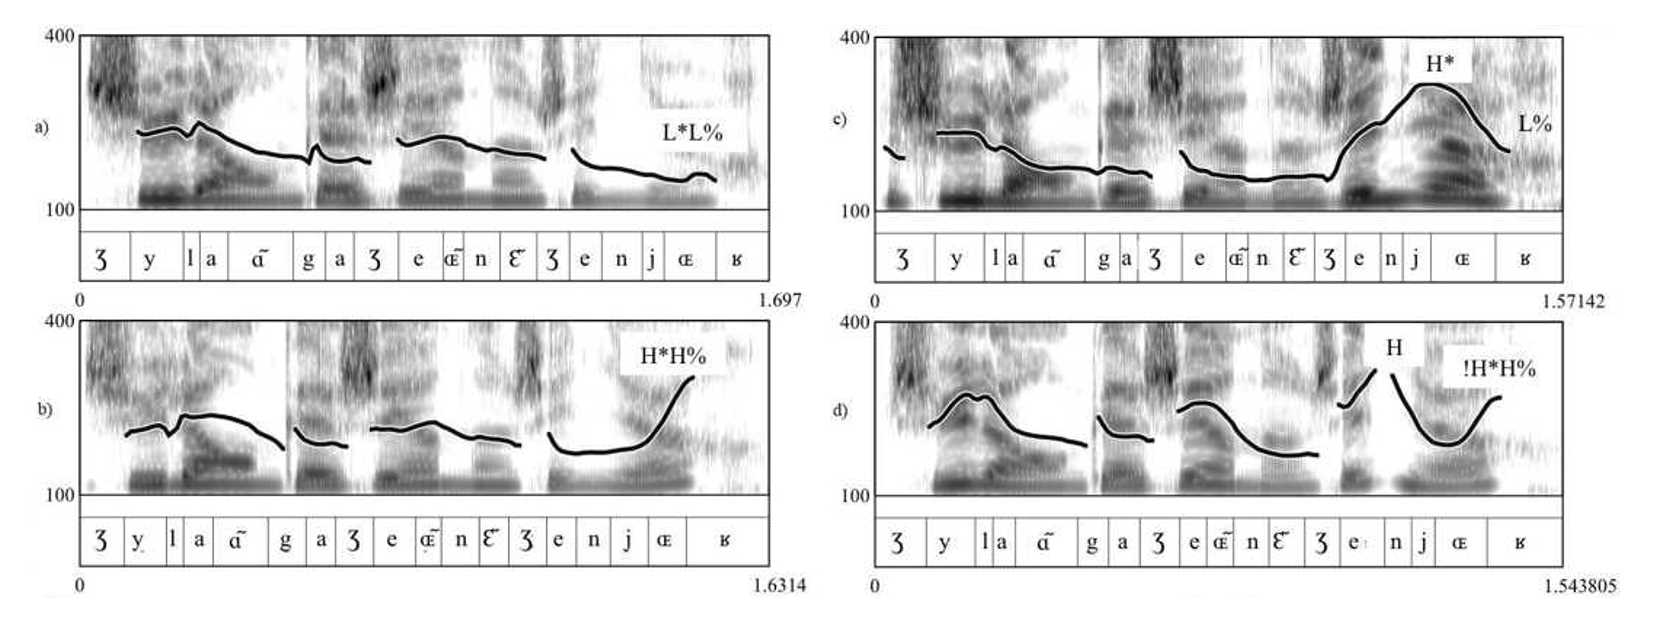
\includegraphics[scale=0.25]{figures/ch10-5.jpg}
  \caption{Four renderings of the utterance \textit{Jules a engagé un ingénieur} `Jules committed an engineer' with the four intonational phrase final contours \citep[adapted from][18]{portesetal2014}: a) L*L\%, b) H*H\%, c) H*L\% and d) H+!H*H\%.}
  \label{fig5}
\end{figure}

On the basis of a theory initiated by \citet{beymar2007}, \citet{portesetal2014} proposed that the meaning of the four contours shown above can be accounted for by using three distinctive features, i.e., \textit{speaker commitment}, \textit{attitude attribution} to the addressee (does the addressee agree or disagree with the speaker?) and \textit{call on addressee}'s next move (a verbal answer, an acknowledgement, another behaviour?). If intonational contours can make public speaker's projections about beliefs attributed to the addressee and the addressee's next move, the latter should dialectically reflect these projections of the speaker in reacting to them. Specifically, in the above study participants were asked to match a declarative sentence bearing one of the four contours with one of four possible meanings summarized in \tabref{table1}.

\begin{sidewaystable}
\begin{tabularx}{\textwidth}{lll}
\lsptoprule
Contour & Pototypical Meaning Features & Reaction\\
\midrule
L*L\% & S commits her-/himself to the truth of $p$ & \textit{J'en prends note} \\
& S signals that (s)he anticipates no disagreement from & `I get it' \\
& A (about $p$) & A acknowledged that S has no disagreement \\
& S proposes to A to update CG with $p$ & about $p$ and that $p$ can be added to the CG \\
\midrule
H*H\%& S signals that (s)he doesn't commit to $p$ & \textit{J'en sais rien} \\
& S signals that (s)he attributes a belief about $p$ to A (that & `I've no idea'\\
& $p$ or $\neg p$) & \multirow{2}{*}{Contradicts S's attribution to A} \\
& S proposes to A to commit to $p$ or to commit to $\neg p$ & \\
\midrule
H*L\% & S commits her-/himself to $p$ & \textit{Tu dois avoir raison} \\
& S signals that (s)he anticipates a disagreement from A:  & `I guess you're right' \\
& S signals that (s)he attributes to A the belief that $\neg p$  & Acknowledgement of S's commitment \\
& S proposes to A to update CG with $p$ & Remaining potential disagreement of A \\
\midrule
H+!H*H\% & S signals that (s)he does not commit to $p$ & \textit{Si, si, je t'assure} \\
& S anticipates a disagreement from A: S signals that & `No, really, it's true' \\
& (s)he attributes to A the belief that $p$) & Comments both on S's disagreement and \\
& S proposes to A either to commit to $p$ or to commit & on the confirmed commitment of A\\
& to $\neg p$ & \\
\lspbottomrule
\end{tabularx}
\caption{Proposed intonation contour meanings designed using the three features proposed by \citet{beymar2007}, and associated reactions \citep[from][]{portesetal2014}.}
\label{table1}
\end{sidewaystable}

Results showed that participants very robustly matched the intonation they heard with the hypothesized reaction for three of the contours (but not for the H*L\%), indicating a promising way to investigate fine grained intonational meaning. As for H*L\%, \citet{portesryle2014} reports a corpus investigation dedicated to its meaning, possibly more sensitive to context and better perceived in presence of a real potentially opposing addressee.

One of these four French intonation contours, the rise-fall-rise H+!H*H\%, was also investigated in a production study \citep{MiPorCham-Lav2016}. In this study, participants had to read a declarative question matched with a negatively biased context eliciting incredulity or matched with a neutral context eliciting an unbiased yes-no question. The questions matching the negatively biased context were produced with the H+!H* pitch accent in 62\% of the cases and with H* in the remaining 38\%. Conversely, the questions matching the neutral context were produced with H* in 97\% of the cases, with 3\% of H+!H*. This result demonstrates that the negative bias was mainly conveyed by the choice of the pitch accent. If we relate this result to the proposal by \citet{portesetal2014}, it appears that the semantic feature \textit{attribution of intention} (agreement/disagreement) should be conveyed by pitch accent choice in French, as proposed by \citet{Portes2015IsIM}. Therefore, the other two features (i.e. speaker commitment and call on addressee), could be jointly conveyed by boundary tones.

\largerpage
An important observation is that, in the negatively biased context, H+!H* was followed by a rise attributed to an H\% boundary tone in 69,4\% of the productions. However, the remaining 30,6\% exhibited a fall that has been interpreted as a L\%. This variability may in fact be explained by a truncation of the H\% boundary tone due to lack of segmental space. This hypothesis remains to be further investigated. If confirmed, this would be a strong piece of evidence that phonological constraints, internal to the intonational system of a language, play an important role in observed variability.

A more striking variability is the production of 38\% H*H\% patterns in the negatively biased context. One possible explanation is that the mere rise expresses mirativity (surprise) in that context, while the H+!H*H\% contours rather express incredulity. Indeed, a surprise meaning may also convey a negative speaker bias even if it is to a lesser degree. One may further speculate that there could be an additional prosodic distinction affecting H*H\% depending on whether it appears in the neutral context or in the negatively biased context: a pitch range variation would certainly be a good candidate. This nuance of meaning hence remains to be better studied in French and other languages.

To conclude this section, several studies on French intonational meaning in the last two decades have contributed to explore an approach where detailed accounts both of intonational form in a phonological approach and of intonational meaning in a semantic perspective allow to give evidence in favour of a possible compositionality of intonational meaning. Such an approach deserves to be refined and enriched by a better understanding of the observed variation, an issue that will be developed in the following section.


\section{Variability in intonational meaning}\label{sec:04:4}
A further point to be addressed is the role of individual variability in both the encoding and decoding of intonational meaning. Within the last decade, the issue of variability has become central in phonetic studies, both at the segmental and at the prosodic level. The sources of such variability can be related to two main factors, i.e., environmental and cognitive factors \citep{kidd2018aa}. More specifically, speech has been found to vary as a function of gender and sexual orientation, socio-economic status, exposure to specific language input as well as cognitive (affecting also neurotypical populations) and emotional states (see \citealt{pierrehumbert2016aa} and \citealt{yu2019aa} for a review of these issues).

Variability in the use of intonation has been found both in production and perception. With specific reference to Italian, the study by Gili Fivela and colleagues \citep{Fivelaetal15} investigated intonation production in several cities and described the general situation as a ``mixing of patterns'', reporting that despite the inter- and intra-variety variability, similar patterns are easily found across Italy, also in geographically distant cities. The authors attribute these findings to factors of socio-political nature, which have an effect that is larger than the individual speaker, e.g. internal migration and the influence of the language of media broadcastings. Recent studies have linked intonational variation in production to individual-specific choices. Great importance has been given to the role of exposure to non-native dialects: while the distribution of polar question tunes can be linked to specific meanings, individual speakers are found to behave very differently from each other as a function of the input they were exposed to throughout their lives, e.g. by having a non-SI parent \citep{orrico19, orrico2020ab}.

The impact of linguistic input on linguistic behaviour at the individual level has also been observed in perception. Both \citet{Orrico+2020} and \citet{orrico2022} have considered the role of past linguistic experience in the attribution of bias-related meanings conveyed by SI question tunes. Taken together, these studies show that the effect of having been exposed for a long time to non-native input (either a foreign language or a non-native dialect of the same language) has a major impact on the way listeners extrapolate tune information. Crucially, the two studies show that the effect is visible at different levels, both at a coarse-grained level – i.e., by asking which phonological elements are considered to primarily convey the bias-related meaning – and at a finer phonetic level – i.e., how gradual variation in pitch span affects the interpretation of question meaning. Interestingly, the general picture yielded by these investigations is that exposure affects the extent to which listeners rely on specific tonal cues to interpret meanings. Indeed, \citet{orrico2022} reported that the exposed population discarded the role of boundary tones and relied only on pitch accents. Similarly, \citet{Orrico+2020} reported that manipulations in the span of pitch accents were interpreted in a coarser way by exposed listeners.

Similar investigations have also been carried out for French. A recent study by \citet{portesgerman2019} has in fact addressed the issue of how listeners manage intonation-meaning mappings in case of exposure to different regional varieties. They reported a study in which a rise-fall tune in French was interpreted not only on the basis of the context in which it is produced, but also of the presence of extralinguistic cues to the specific geographical location. Note that this rise-fall tune is ambiguous since it is used in Continental French to encode a statement and in Corsican French to encode a polar question. In their model, tune-meaning mappings are stored in the listeners' mental representation in association with a contextual label (in this case, Continental or Corsican French), in a way that contextual cues can determine which mapping is relevant in the situation and therefore activated. Crucially, the extent to which the contextual cue is functional to the correct interpretation of the meaning is strictly linked to the amount of relative exposure to the two varieties, with the greatest advantage predicted for listeners with a balanced exposure to the two systems \citep{germanportes2020}.

A further source of variation of the tune-meaning mapping concers listeners' cognitive states. Recent research has pointed out that the degree of cognitive and emotional empathy determines the way in which intonational meaning is processed. In an eye-tracking study, \citet{esteveetal2020} show that the interpretation of ambiguous utterances by French listeners varies as a function of the empathy skills of the listeners: while listeners with low empathy skills show a weaker reliance on prosodic information leading to the disambiguation of lexical items, listeners with higher empathy skills attended more closely to prosodic information and showed a higher sensitivity to the possible meanings conveyed by the tonal contour. Similarly, \citet{Orrico+2020} introduced the degree of empathy skills in their experimental setting, reporting that empathic listeners were more attentive to fine tonal modifications and to the way they are used to encode meanings than the low-empathy group. Interestingly, empathy was also found to affect the role of exposure to other linguistic systems. Specifically, \citet{Orrico+2020} found that the perceptual change as a result to exposure to non-native language was strongest in high-empathy listeners. These results provide an impression of the extreme sensitivity of intonational meaning to a number of different factors, which should be taken into account when conducting research on this issue.

\section{Which dimensions of bias in questions are conveyed by intonation?}\label{sec:04:5}
This chapter has reported a discussion on the general role of intonation in the conveyance of information linked to question bias. The idea is that the speaker aims at signalling that s/he is not completely ignorant with respect to the propositional content of the utterance. The findings reported here also allow to characterize the dimensions over which intonation operates in the expression of these meanings.

First, intonation serves the role of signalling that the speaker has his/her own beliefs with respect of the question being asked and, additionally, it allows for finer specifications of the type and strength of the belief as well as how they are positioned relative the interlocutor's beliefs. Intonation is hence also involved in the conveyance of the presence of speaker bias, through the expression of speaker commitment. This function of intonation are attributed to the type of pitch accent in nuclear position in Italian, with the L+H* early rise conveying that the speaker is committing to the surface proposition within the question, as opposed to the L*+H late rise, which signals that the speaker is not making a commitment toward the truth of the proposition. On the contrary, French exploits boundary tones to encode this meaning, with L\% boundaries being linked to the expression of speaker commitment. Moreover, both languages make use of intonational cues to encode negative bias, by signalling that some piece of information is in contrast with what the speaker previously believed to be true. On one hand, this meaning is assigned to pitch accent type in French, specifically through the use of a H+!H*. On the other hand, Salerno Italian conveys this meaning by modulating the pitch span within the L+H* rise, with a narrower span in case of negative bias. Moreover, the pitch span feature is also exploited by Salerno Italian to encode information about the relative strength of speaker commitment: a wider excursion would allow signalling that the expectation for a positive answer to the question is significantly higher. Finally, we show that intonation was also involved in the attribution of commitment from the speaker to the addressee, which is again encoded through the type of pitch accent in French. As for Italian, an impressionistic analysis of the data collected suggests that the meaning of commitment attribution might be conveyed by boundary tones. More specifically, the presence of a H\% boundary in questions might signal that the speaker is attributing the addressee the role of source of the commitment and, therefore, the commitment expressed by the speaker is only tentative and dependent on the addressee's ratification.

Taken together, the findings reported here for both Italian and French allow us to make general considerations about intonational meaning. On the one hand, intonational meaning is not universal. Specifically, although intonation might have a similar role in different languages, the way in which specific meanings are encoded within an intonation contour is language-specific. Moreover, both French and Italian would extract similar functions from intonation as related to the expression of meanings relative to question bias, i.e., signalling the presence of bias, specifying the position of the speaker relative to the proposition and to the addressee and, possibly, defining the source of the commitment. Nevertheless, the way in which the meanings are grammaticalized within the two languages appears to be different. Note that differences might also be found within different varieties of the same language. Recall, for example, the differences in the meaning assigned to the rise-fall in Continental and Corsican French. Furthermore, lack of universality is also found as far as fine phonetic modifications are concerned. For instance, the incredulity conveyed by narrower pitch span in Salerno Italian is not found in all other varieties of the same language. In Bari Italian, for example, the same meaning is conveyed through a wider span within the pitch accent \citep{savino2011aa}.

The link between pitch range, information and pragmatic meanings, as also reported in \sectref{sec:04:2}, has been reported in several languages. Among these, \citet{savino2011aa} and \citet{crocco2016aa} reported the role of pitch excursion in modulating the meaning of a question in two varieties of Italian. \citet{hirschberg92} also found that information relative to pitch range was instrumental in determining the difference between an incredulous and an uncertain reading of the rise-fall-rise contour in English. Further, \citet{vanrell2011aa} and \citet{borras-Comes2014aa} showed that , in Catalan, a different scaling of the peak within the pitch accent is a crucial cue for discriminating across linguistic categories, both in production and perception. Both the above studies as well as the findings reported here for Salerno Italian allow to clarify yet another controversial issue of intonational meaning, specifically which are the tonal elements responsible for meaning conveyance. While information relative to pitch range and level beyond the two phonological discrete tones (L and H) is often discarded both in the analysis of intonation and its meaning, these studies point out that gradual information relative to pitch height might actually be involved in the expression of pragmatic meanings and therefore deserve to be acknowledged and accounted for in intonational meaning models. Nevertheless, the way in which this type of information should be integrated in existing models is not yet proposed here, especially considering that most of the models proposed seem to advocate for the absence of a direct link between phonetic information and pragmatics/semantics, given phonology mediation. One possibility, which appears to be compatible with findings in \citet{Orrico+2020} for Salerno Italian, is that pitch span manipulation is not meaningful \textit{per se}, though it modulates the core meaning of the pitch accent (or the tonal discrete element it modifies). For instance, in the case of L+H*, while its core meaning would be committing the speaker to some proposition, a pitch span modification would modulate the speaker confidence to that commitment and, in this specific case, the degree of bias. An intonational meaning model allowing for these types of gradual modification of meaning would, in turn, require that also the pragmatic side should acquire a finer granularity.

Finally, the data reported above suggest that the way intonation is linked to pragmatic meanings is extremely sensitive to various sources of variation, making the investigation of these issues both a theoretical and a methodological challenge. On the theoretical side, one major implication of this issue is relative to how we even understand meanings conveyed through intonation. As reported above, two studies that address this issue are \citet{portesgerman2019} and \citet{germanportes2020} reported in \sectref{sec:04:4}, in which the authors propose an exemplar-based model in which intonational contours are stored with contextual-specific meanings and retrieved when needed during communication. In general, very little has been done as far as processing of intonation in variable contexts is concerned. Some experimental studies have been conducted (among others \citealt{kurumada2014or, roettger2020aa}), which, together with experimental evidence discussed in this chapter, reinforce the idea that we, as language users, are extremely adaptive and, when put before unprecedented or variable situations, rapidly adapt and change the way the speech input is processed. This should be kept in mind both when we set up experimental procedures to investigate intonational meaning and when we interpret the results.

\section{Conclusion}\label{conclude}
This chapter had the aim of defining the way intonation is used by interlocutors to encode and decode meanings related to bias in polar questions, by reporting on recent studies addressing this specific issue. More specifically, the chapter has focused on three main aspects: the definition of the bias-related meanings that can be conveyed by prosodic cues, the elements of intonation that are exploited to convey those meanings and, finally, the variability that exists in the mapping between intonational cues and meaning expressed within a linguistic community. The investigation reported here concern two Romance languages, French and Salerno Italian, whose intonation has extensively been studied in recent research. The point made here is that intonation plays a crucial role in conveying discourse meaning, by defining, at various levels, the attitude of speakers and listeners towards the propositional content which, in turn, allows for the definition of the meaning of utterances. Nevertheless, several aspects concerning the contribution of intonation are still to be settled, such as the way gradient phonetic information maps onto meanings of semantic nature, the relationship between intonation and other linguistic levels or even gestures, and the role of variability. Future research should aim to provide answers to these questions. 
{\sloppy\printbibliography[heading=subbibliography,notkeyword=this]}
\end{document}
